\documentclass[12 pt, final]{article}
% Imports =====================================================================

\usepackage{amsfonts,amssymb,amsthm,amsmath,mathrsfs,mathtools}
\usepackage{algorithmicx}
\usepackage[plain]{algorithm}
\usepackage[noend]{algpseudocode}
\usepackage{bigstrut}
\usepackage{blkarray}
\usepackage{cancel}
\usepackage{color}
\usepackage{comment}
\usepackage{float}
\usepackage{graphicx}
\usepackage[customcolors]{hf-tikz}
\usepackage{ifdraft}
\usepackage{listings}
\usepackage[framemethod=tikz]{mdframed}
\usepackage[inline]{showlabels}
\usepackage{subcaption}
\usepackage{textcomp}
\usepackage{tikz}
\usepackage{xcolor}
\usepackage{xparse}
\usepackage{url}

% Page setup ==================================================================

\pagestyle{plain} \setlength{\headheight}{0in}
\setlength{\topmargin}{0in} \setlength{\headsep}{0in}
\setlength{\voffset}{0 in} \setlength{\textheight}{9in}
\setlength{\oddsidemargin}{0 in} \setlength{\evensidemargin}{0in}
\setlength{\textwidth}{6.5in} \setlength{\headheight}{0in}
\setlength{\headsep}{0in} \setlength{\hoffset}{0in}
\setlength{\parsep}{6pt}
\setlength{\parskip}{6pt}
\theoremstyle{plain}
\linespread{1.1}

% Environments ================================================================

% Use o for second-level nested itemized.
\renewcommand{\labelitemii}{$\circ$}

% Display labels and color tags.
\newtagform{red}{\color{red}(}{)}
\newtagform{orange}{\color{orange}(}{)}
\newtagform{green}{\color{green}(}{)}
\newtagform{yellow}{\color{yellow}(}{)}
\newtagform{blue}{\color{blue}(}{)}
\newtagform{purple}{\color{purple}(}{)}

\renewcommand{\showlabelfont}{\small\ttfamily\color{orange}}

% Tikzpicture tools
\usetikzlibrary{arrows, automata, backgrounds, calendar, chains, decorations,
    matrix, mindmap, patterns, petri, positioning, shadows, shapes.geometric,
    trees, shapes, decorations.pathreplacing}
\usetikzlibrary{circuits.ee.IEC}

% Theorems
\newtheorem{proposition}{Proposition}
\newtheorem{lemma}{Lemma}
\newtheorem{theorem}{Theorem}
\newtheorem{corollary}{Corollary}
\newtheorem{remark}{Remark}
\newtheorem*{proposition*}{Proposition}
\newtheorem*{lemma*}{Lemma}
\newtheorem*{theorem*}{Theorem}
\newtheorem*{corollary*}{Corollary}
\newtheorem*{remark*}{Remark}

% Problem set
\newenvironment{problems}{\begin{list}{}{\setlength{\itemsep}{12pt}\setlength{\labelwidth}{.5in}\leftmargin=0in}}{\end{list}}
\newcounter{problempart}
\newenvironment{parts}{\begin{list}{$\bullet$}{\setlength{\itemsep}{6pt}\setlength{\parsep}{6pt}\setlength{\parskip}{6pt}\usecounter{problempart}\setlength{\labelwidth}{.5in}\leftmargin=.25in}}{\end{list}}
% \setlist[problems]{leftmargin=1in}

% Equation labeling by section (TODO: by problem).
% \numberwithin{equation}{section}

% Syntax highlighting
\definecolor{brightred}{rgb}{1, 0, 0}           % bright red
\definecolor{red}{cmyk}{0, 1.00, 0.62,0}        % red
\definecolor{blue}{cmyk}{1.00, .34, .0 .02 }    % blue
\definecolor{green}{cmyk}{0.7, 0, 1.0, 0.09 }   % greenish
\definecolor{yellow}{cmyk}{0, 0.16, 1.0, 0}     % yellow
\definecolor{gray}{cmyk}{0, 0, 0, 0.65}         % gray
\definecolor{purple}{cmyk}{.333, .867, 0, .059} % purple
\colorlet{shadecolor}{blue!10}
\colorlet{warning}{red!20!}
\colorlet{warnline}{red}
\colorlet{information}{green!20}
\colorlet{infoline}{green}
\colorlet{codebase}{yellow!5!}
\colorlet{codekeyword}{blue}
\colorlet{codecomment}{green}
\colorlet{codestring}{red}

% Code boxes
\lstset{
  language=Python,
  backgroundcolor=\color{codebase},
  tabsize=4,
  basewidth=.5em,
  rulecolor=\color{yellow},
  basicstyle=\linespread{0.85}\small\ttfamily,    % code text size
  upquote=true,
  columns=fixed,
  extendedchars=true,
  breaklines=true,
  prebreak = \raisebox{0ex}[0ex][0ex]{\ensuremath{\hookleftarrow}},
  frame=lrtb,
  % xleftmargin=0pt,
  % xrightmargin=0pt,
  framesep=4pt,
  framerule=2pt,
  showtabs=false,
  showspaces=false,
  showstringspaces=false,
  morestring=[s]{"""}{"""},
  morestring=[s]{'''}{'''},
  keywordstyle=\color{codekeyword},
  commentstyle=\color{codecomment},
  stringstyle=\color{codestring},
  title=\lstname,
  captionpos=b,
  abovecaptionskip=-5pt,
  belowcaptionskip=-5pt,
  moredelim=[is][\color{black}]{<<}{>>},
  moredelim=[is][\color{red}]{<r<}{>r>},
  moredelim=[is][\color{blue}]{<b<}{>b>},
  moredelim=[is][\color{green}]{<g<}{>g>},
  moredelim=[is][\color{purple}]{<p<}{>p>},
  morekeywords={assert, bytes, self, super, with, as, yield, True, False,
    None, NotImplemented, BaseException, Exception, AssertionError,
    AttributeError, ImportError, IndexError, KeyError, KeyboardInterrupt,
    MemoryError, NameError, NotImplementedError, OSError, OverflowError,
    RecursionError, RuntimeError, StopIteration, SyntaxError,
    IndentationError, TabError, StandardError, SystemError, SystemExit,
    TypeError, ValueError, ZeroDivisionError, IOError, Warning,
    RuntimeWarning, FileExistsError, FileNotFoundError,
    SELECT, FROM, AS, INNER, JOIN, LEFT, OUTER,
    CROSS, ON, WHERE, CASE, IF, MIN, MAX, SUM, AVG, COUNT, TEXT, REAL
  },
  deletekeywords={compile, format}
}

\newcommand{\li}[1]{\lstinline[prebreak=]!#1!}          % Inline code

% Algorithmic environment commands
\lstdefinestyle{pseudo}{basicstyle=\rmfamily,
                        upquote=true,
                        keywordstyle=\color{black}\bfseries,
                        commentstyle=\color[rgb]{0.133,0.545,0.133},
                        stringstyle=\color[rgb]{0.627,0.126,0.941},
                        }
\newcommand{\pseudoli}[1]{\lstinline[style=pseudo]!#1!}
\NewDocumentCommand\allocate{m+g}{                      % Empty array
  \IfNoValueTF{#2}
    {\mathrm{empty}(#1)}                                % 1 dimension
    {\mathrm{empty}(#1, #2)}                            % 2 dimensions
}
\NewDocumentCommand\zeros{m+g}{                         % Zero array
  \IfNoValueTF{#2}
    {\mathrm{zeros}(#1)}
    {\mathrm{zeros}((#1, #2))}
}
\newcommand{\Id}[1]{\mathrm{Id}(#1)}                    % Identity array
\newcommand{\makecopy}[1]{\mathrm{copy}(#1)}            % Copy an array
\newcommand{\shape}[1]{\mathrm{shape}(#1)}
\newcommand{\size}[1]{\mathrm{size}(#1)}

% Shortcuts ===================================================================

% Bold letters / numbers
\newcommand{\bfa}{\mathbf{a}}
\newcommand{\bfA}{\mathbf{A}}
\newcommand{\bfb}{\mathbf{b}}
\newcommand{\bfB}{\mathbf{B}}
\newcommand{\bfc}{\mathbf{c}}
\newcommand{\bfC}{\mathbf{C}}
\newcommand{\bfd}{\mathbf{d}}
\newcommand{\bfD}{\mathbf{D}}
\newcommand{\bfe}{\mathbf{e}}
\newcommand{\bfE}{\mathbf{E}}
\newcommand{\bff}{\mathbf{f}}
\newcommand{\bfF}{\mathbf{F}}
\newcommand{\bfg}{\mathbf{g}}
\newcommand{\bfG}{\mathbf{G}}
\newcommand{\bfh}{\mathbf{h}}
\newcommand{\bfH}{\mathbf{H}}
\newcommand{\bfi}{\mathbf{i}}
\newcommand{\bfI}{\mathbf{I}}
\newcommand{\bfj}{\mathbf{j}}
\newcommand{\bfJ}{\mathbf{J}}
\newcommand{\bfk}{\mathbf{k}}
\newcommand{\bfK}{\mathbf{K}}
\newcommand{\bfl}{\boldsymbol{\ell}}
\newcommand{\bfL}{\mathbf{L}}
\newcommand{\bfm}{\mathbf{m}}
\newcommand{\bfM}{\mathbf{M}}
\newcommand{\bfn}{\mathbf{n}}
\newcommand{\bfN}{\mathbf{N}}
\newcommand{\bfo}{\mathbf{o}}
\newcommand{\bfO}{\mathbf{O}}
\newcommand{\bfp}{\mathbf{p}}
\newcommand{\bfP}{\mathbf{P}}
\newcommand{\bfq}{\mathbf{q}}
\newcommand{\bfQ}{\mathbf{Q}}
\newcommand{\bfr}{\mathbf{r}}
\newcommand{\bfR}{\mathbf{R}}
\newcommand{\bfs}{\mathbf{s}}
\newcommand{\bfS}{\mathbf{S}}
\newcommand{\bft}{\mathbf{t}}
\newcommand{\bfT}{\mathbf{T}}
\newcommand{\bfu}{\mathbf{u}}
\newcommand{\bfU}{\mathbf{U}}
\newcommand{\bfv}{\mathbf{v}}
\newcommand{\bfV}{\mathbf{V}}
\newcommand{\bfw}{\mathbf{w}}
\newcommand{\bfW}{\mathbf{W}}
\newcommand{\bfx}{\mathbf{x}}
\newcommand{\bfX}{\mathbf{X}}
\newcommand{\bfy}{\mathbf{y}}
\newcommand{\bfY}{\mathbf{Y}}
\newcommand{\bfz}{\mathbf{z}}
\newcommand{\bfZ}{\mathbf{Z}}

\newcommand{\e}{\bfe}
\newcommand{\E}{\bfE}
\newcommand{\f}{\bff}
\newcommand{\F}{\bfF}
\newcommand{\g}{\bfg}
\newcommand{\G}{\bfG}
\newcommand{\h}{\bfh}
\newcommand{\w}{\bfw}
\newcommand{\W}{\bfW}
\newcommand{\x}{\bfx}
\newcommand{\X}{\bfX}
\newcommand{\y}{\bfy}
\newcommand{\Y}{\bfY}
\newcommand{\z}{\bfz}
\newcommand{\Z}{\bfZ}
\newcommand{\0}{\mathbf{0}}

% Bold Greek letters
\newcommand{\bfalpha}{\boldsymbol{\alpha}}
\newcommand{\bfbeta}{\boldsymbol{\beta}}
\newcommand{\bfgamma}{\boldsymbol{\gamma}}
\newcommand{\bfdelta}{\boldsymbol{\delta}}
\newcommand{\bfepsilon}{\boldsymbol{\epsilon}}
\newcommand{\bfzeta}{\boldsymbol{\zeta}}
\newcommand{\bfeta}{\boldsymbol{\eta}}
\newcommand{\bftheta}{\boldsymbol{\theta}}
\newcommand{\bfiota}{\boldsymbol{\iota}}
\newcommand{\bfkappa}{\boldsymbol{\kappa}}
\newcommand{\bflambda}{\boldsymbol{\lambda}}
\newcommand{\bfmu}{\boldsymbol{\mu}}
\newcommand{\bfnu}{\boldsymbol{\nu}}
\newcommand{\bfxi}{\boldsymbol{\xi}}
\newcommand{\bfomicron}{\boldsymbol{\omicron}}
\newcommand{\bfpi}{\boldsymbol{\pi}}
\newcommand{\bfrho}{\boldsymbol{\rho}}
\newcommand{\bfsigma}{\boldsymbol{\sigma}}
\newcommand{\bftau}{\boldsymbol{\tau}}
\newcommand{\bfupsilon}{\boldsymbol{\upsilon}}
\newcommand{\bfphi}{\boldsymbol{\phi}}
\newcommand{\bfchi}{\boldsymbol{\chi}}
\newcommand{\bfpsi}{\boldsymbol{\psi}}
\newcommand{\bfomega}{\boldsymbol{\omega}}
\newcommand{\bfvarepsilon}{\boldsymbol{\varepsilon}}
\newcommand{\bfvartheta}{\boldsymbol{\vartheta}}
\newcommand{\bfvarkappa}{\boldsymbol{\varkappa}}
\newcommand{\bfvarpi}{\boldsymbol{\varpi}}
\newcommand{\bfvarrho}{\boldsymbol{\varrho}}
\newcommand{\bfvarphi}{\boldsymbol{\varphi}}
\newcommand{\bfvarsigma}{\boldsymbol{\varsigma}}
\newcommand{\bfGamma}{\boldsymbol{\Gamma}}
\newcommand{\bfDelta}{\boldsymbol{\Delta}}
\newcommand{\bfTheta}{\boldsymbol{\Theta}}
\newcommand{\bfLambda}{\boldsymbol{\Lambda}}
\newcommand{\bfUpsilon}{\boldsymbol{\Upsilon}}
\newcommand{\bfXi}{\boldsymbol{\Xi}}
\newcommand{\bfPhi}{\boldsymbol{\Phi}}
\newcommand{\bfPi}{\boldsymbol{\Pi}}
\newcommand{\bfPsi}{\boldsymbol{\Psi}}
\newcommand{\bfSigma}{\boldsymbol{\Sigma}}
\newcommand{\bfOmega}{\boldsymbol{\Omega}}

% Common spaces
\renewcommand{\AA}{\mathbb{A}}
\newcommand{\BB}{\mathbb{B}}
\newcommand{\CC}{\mathbb{C}}                    % complex numbers
\newcommand{\DD}{\mathbb{D}}
\newcommand{\EE}{\mathbb{E}}
\newcommand{\FF}{\mathbb{F}}                    % the complex or real field
\newcommand{\GG}{\mathbb{G}}
\newcommand{\HH}{\mathbb{H}}
\newcommand{\II}{\mathbb{I}}
\newcommand{\JJ}{\mathbb{J}}
\newcommand{\KK}{\mathbb{K}}
\newcommand{\LL}{\mathbb{L}}
\newcommand{\MM}{\mathbb{M}}
\newcommand{\NN}{\mathbb{N}}                    % natural numbers
\newcommand{\OO}{\mathbb{O}}
\newcommand{\PP}{\mathbb{P}}
\newcommand{\QQ}{\mathbb{Q}}
\newcommand{\RR}{\mathbb{R}}                    % real numbers
\renewcommand{\SS}{\mathbb{S}}
\newcommand{\TT}{\mathbb{T}}
\newcommand{\UU}{\mathbb{U}}
\newcommand{\VV}{\mathbb{V}}
\newcommand{\WW}{\mathbb{W}}
\newcommand{\XX}{\mathbb{X}}
\newcommand{\YY}{\mathbb{Y}}
\newcommand{\ZZ}{\mathbb{Z}}                    % integers

% Integrals
\newcommand{\dr}{\:dr}                          % 1-d integral in r
\newcommand{\ds}{\:ds}                          % 1-d integral in s
\newcommand{\dt}{\:dt}                          % 1-d integral in t
\newcommand{\dx}{\:dx}                          % 1-d integral in x
\newcommand{\dX}{\:d\bfx}                       % n-d integral in x
\newcommand{\dy}{\:dy}                          % 1-d integral in y
\newcommand{\dY}{\:d\bfy}                       % n-d integral in y
\newcommand{\dz}{\:dz}                          % 1-d integral in z
\newcommand{\dZ}{\:d\bfz}                       % n-d integral in z
\newcommand{\dA}{\:dA}                          % area integral
\newcommand{\dS}{\:dS}                          % surface integral
\newcommand{\dV}{\:dV}                          % volume integral
\newcommand{\dXi}{\:d\bfxi}                     % Lagrangian volume integral

% Matrix operations
\newcommand{\inv}{^{-1}}                        % matrix inverse
\newcommand{\trp}{^{\mathsf T}}                 % matrix transpose
\newcommand{\invtrp}{^{\mathsf{-T}}}            % matrix inverse transpose
\newcommand{\hrm}{^{\mathsf H}}                 % matrix Hermitian
\newcommand{\invhrm}{^{\mathsf{-H}}}            % matrix inverse Hermitian

% Inner product angle braces
\newcommand{\<}{\left\langle}
\renewcommand{\>}{\right\rangle}

% Other
\newcommand{\weakto}{\rightharpoonup}           % weak convergence
\DeclareMathOperator*{\esssup}{ess\,sup}        % essential supremum
\DeclareMathOperator*{\argmax}{arg\,max}        % argmax
\DeclareMathOperator*{\argmin}{arg\,min}        % argmin
\renewcommand{\CancelColor}{\color{lightgray}}  % color for \cancelto{}{}.
\newcommand{\TODO}[1][]{\textcolor{brightred}{\text{\textbf{TODO}#1}}}

\usepackage{xcolor}
\usepackage{multirow}
\renewcommand{\t}{\texttt}
\renewcommand{\d}{\times}
% https://tex.stackexchange.com/questions/133795/change-the-color-of-background-of-code-of-matlab
 \renewcommand\labelitemii{\textendash}
 \def \checkmark{\tikz\fill[scale=0.4](0,.35) -- (.25,0) -- (1,.7) -- (.25,.15) -- cycle;} 
\begin{document} % ============================================================

% Title
\noindent\textsc{
CSE 380 Fall 2020
\hfill
Project 2
\hfill
Shreyas Gaikwad (sg49969)}

% Authors (alphabetical by last name, reverse alphabetical by first name o_O)
\begin{center}
\Large{\textbf{Modeling Document}}
\end{center}

\begin{itemize}
    \item \textbf{Governing Equations}
        \begin{align}
            -k\nabla^2 T(x,y) &= q(x,y) \:\text{ in }\: \Omega \label{eq1}\\
            T(x,y) &= T_{masa} (x,y) \text{ on }\: \partial\Omega \nonumber 
        \end{align}
        where,
        \begin{align*}
            \Omega &\:\text{ is a 2D bounded domain}\\
            \partial\Omega &\:\text{ is the boundary of the domain}\\
            T &\:\text{ is the material's temperature field}\\
            q &\:\text{ is the heat source term}\\
            k &\:\text{ is the thermal conductivity}
        \end{align*}
        We have the Dirichlet boundary conditions.
        
    \item \textbf{Assumptions}
        \begin{itemize}
            \item The thermal conductivity is assumed to be constant.
            \item We assume a square domain $\Omega = \{\:(x,y) : x \in [0,L], y \in [0,L]\:\}$ for the 2D case. For 1D, it will obviously be a line $\Omega = \{\:(x,y) : x \in [0,L]\:\}$
            \item Dirichlet boundary condition is assumed at the boundaries
            \item For the fourth order scheme, we assume that the values at the points adjacent to the boundary points are known from the \texttt{MASA} solution. This is to reduce the cumbersome effort required to come up with different schemes at the boundary.
            \item For the 2D case we assume symmetrical discretization i.e. the number of grid points in both directions are the same and $\Delta x = \Delta y = h$.
        \end{itemize}
    \item \textbf{Nomenclature for discretization}
    Our numerical methods are all node based (as will be reiterated later).
        \begin{itemize}
            \item 1D We have $(N+1)$ points $\{x_0,x_1,x_2,\hdots x_N\}$ in the x-direction with $x_i=i\Delta x$, where $\Delta x = L/N$
                
            \item 2D We have $(N+1)$ points $\{x_0,x_1,x_2,\hdots x_N\}$ in the x-direction with $x_i=i\Delta x$, where $\Delta x = L/N = h$ and $(N+1)$ points $\{y_0,y_1,y_2,\hdots y_N\}$ in the y-direction with $y_j=j\Delta y$, where $\Delta y = L/N = h$. Hence, we have a $(N+1) \times (N+1)$ grid. 
            
            \item $i$ is always associated with the indexing in x-direction and $j$ is always associated with the indexing in y-direction.
            
            \item $T(x_i,y_j)$ is given the shorthand notation $T(i,j)$ and $q(x_i,y_j)$ is given the shorthand notation $q(i,j)$
            \item The composite index for 2D grid is given by $k = i + (N+1)j$.
        \end{itemize}
    \item \textbf{Numerical Method}
    
        Our numerical methods are all node based (as will be reiterated later).
        \begin{itemize}
            \item \textbf{$2^{\text{nd}}$ order finite difference approximation}
            
            \textbf{Definition}
            \begin{align*}
                \frac{\partial^2 T}{\partial x^2} \approx \frac{T(x+\Delta x)-2T(x)+T(x-\Delta x)}{\Delta x^2} + \mathcal{O}(\Delta x^2)
            \end{align*}
            \textbf{Discretized heat equation}
            \begin{enumerate}
            
                \item 1D
                \begin{align}
                \begin{cases}    -k\left(\frac{T(i+1)-2T(i)+T(i-1)}{\Delta x^2}\right) + \mathcal{O}(\Delta x^2) = q(i), \:\: i \:\in \{1,2,3,\hdots, N-1\}\\
                    T(0) = T_{masa} (0) \:\text{ and }\: T(N) = T_{masa} (L) \label{eq2}
                \end{cases}
                \end{align}
                
                \item 2D
                \begin{align}
                \begin{cases}    -k\left(\frac{T(i+1,j)-2T(i,j)+T(i-1,j)}{h^2}\right) -k\left(\frac{T(i,j+1)-2T(i,j)+T(i,j-1)}{h^2}\right) \\
                +\mathcal{O}(h^2)= q(i,j),\:\: i \:\in \{1,2,3,\hdots, N-1\}\:\:j \:\in \{1,2,3,\hdots, N-1\}\\\\
                T(i,j) = T_{masa} (x_i,y_j) \:\text{ for }\: i \:\in \{0,N\},\:j\in\{0, 1, 2, \hdots , N\}\\
                T(i,j) = T_{masa} (x_i,y_j) \:\text{ for }\: i \:\in \{0, 1, 2, \hdots , N\},\:j\in\{0,N\} \label{eq3}
                \end{cases}
                \end{align}
                
            \end{enumerate}
            \item \textbf{$4^{\text{th}}$ order finite difference approximation}
            
            \textbf{Definition}
            \begin{align*}
                \frac{\partial^2 T}{\partial x^2} \approx \frac{-T(x-2\Delta x) + 16 T(x-\Delta x) - 30 T(x) + 16 T(x+\Delta x) - T(x+2\Delta x)}{12 \Delta x^2}+ \mathcal{O}(\Delta x^4)
            \end{align*}            
            \textbf{Discretized heat equation}
            
            We have Dirichlet boundary conditions at both the boundary points and adjacent to boundary points.
            \begin{enumerate}
                \item 1D
                \begin{align}
                \begin{cases}
                    -k\left(\frac{-T(i-2) + 16 T(i-1) - 30 T(i) + 16 T(i+1) - T(i+2)}{12 \Delta x^2}\right)+ \mathcal{O}(\Delta x^4) = q(i), \:\: i \:\in \{2,3,\hdots, N-2\}\\
                    T(i) = T_{masa} (x_i), \:\: i \:\in \{0,1,N-1,N\} \label{eq4}
                \end{cases}
                \end{align}
                \item 2D
                
                \begin{align}
                \begin{cases}
                    -k\left(\frac{-T(i-2,j) + 16 T(i-1,j) - 30 T(i,j) + 16 T(i+1,j) - T(i+2,j)}{12 h^2}\right)\\ -k\left(\frac{-T(i,j-2) + 16 T(i,j-1) - 30 T(i,j) + 16 T(i,j+1) - T(i,j+2)}{12 h^2}\right)+ \mathcal{O}(h^4) = q(i,j),\\ \:\: i \:\in \{2,\hdots, N-2\}, j \:\:\in \{2,\hdots, N-2\}\\\\
                    T(i,j) = T_{masa} (x_i,y_j) \:\text{ for }\: i \:\in \{0,1,N-1,N\},\:j\in\{0, 1, 2, \hdots , N\}\\
                    T(i,j) = T_{masa} (x_i,y_j) \:\text{ for }\: i \:\in \{0, 1, 2, \hdots , N\},\:j\in\{0,1,N-1,N\}\label{eq5}
                \end{cases}
                \end{align}
            \end{enumerate}
        \end{itemize}
    \item \textbf{Mesh diagrams}
    
    Our schemes are node based.
    \begin{enumerate}
        \item 1D
        
        \hspace{2cm}\begin{tikzpicture}[scale=0.4, vertices/.style={draw, fill=black, circle, inner sep=0.5pt}]
        \node[vertices, label={$x_0$}] (a) at (0,0) {};
        \node[vertices, label={$x_1$}] (b) at (3,0) {};
        \node[vertices, label={$x_2$}] (c) at (6,0) {};
        \node[vertices, label={$x_{i}$}] (d) at (12,0) {};
        \node[vertices, label={$x_{N-1}$}] (e) at (21,0) {};
        \node[vertices, label={$x_{N}$}] (f) at (24,0) {};
        \foreach \to/\from in
        {a/b,b/c,e/f} \draw [-] (\to)--(\from);
        \foreach \to/\from in
        {c/d,d/e} \draw [dashed]     (\to)--     (\from);
        \draw[|<->|] (0,-2) to (24,-2);
        \draw[|<->|] (3,1.5) to (6,1.5);
        \path (0,-1.3) -- (24,-1.3) node[pos=0.5]  {$L$};
        \path (3,2.3) -- (6,2.3) node[pos=0.5]  {$\Delta x$};
        \end{tikzpicture}
        \item 2D
       \end{enumerate}     
        \begin{tikzpicture}[scale=0.4, vertices/.style={draw, fill=black, circle, inner sep=0.5pt}]
        \node[vertices, label={$(x_0,y_0)$}] (a) at (0,0) {};
        \node[vertices, label={$(x_1,y_0)$}] (b) at (5,0) {};
        \node[vertices, label={$(x_2,y_0)$}] (c) at (10,0) {};
        \node[vertices, label={$(x_i,y_0)$}] (d) at (20,0) {};
        \node[vertices, label={$(x_{N-1},y_0)$}] (e) at (30,0) {};
        \node[vertices, label={$(x_{N},y_0)$}] (f) at (35,0) {};
        
        \node[vertices, label={$(x_0,y_1)$}] (g) at (0,5) {};
        \node[vertices, label={$(x_1,y_1)$}] (h) at (5,5) {};
        \node[vertices, label={$(x_2,y_1)$}] (i) at (10,5) {};
        \node[vertices, label={$(x_i,y_1)$}] (j) at (20,5) {};
        \node[vertices, label={$(x_{N-1},y_1)$}] (k) at (30,5) {};
        \node[vertices, label={$(x_{N},y_1)$}] (l) at (35,5) {};
        
        \node[vertices, label={$(x_0,y_2)$}] (m) at (0,10) {};
        \node[vertices, label={$(x_1,y_2)$}] (n) at (5,10) {};
        \node[vertices, label={$(x_2,y_2)$}] (o) at (10,10) {};
        \node[vertices, label={$(x_i,y_2)$}] (p) at (20,10) {};
        \node[vertices, label={$(x_{N-1},y_2)$}] (q) at (30,10) {};
        \node[vertices, label={$(x_{N},y_2)$}] (r) at (35,10) {};        
        
        \node[vertices, label={$(x_0,y_j)$}] (s) at (0,20) {};
        \node[vertices, label={$(x_1,y_j)$}] (t) at (5,20) {};
        \node[vertices, label={$(x_2,y_j)$}] (u) at (10,20) {};
        \node[vertices, label={$(x_i,y_j)$}] (v) at (20,20) {};
        \node[vertices, label={$(x_{N-1},y_j)$}] (w) at (30,20) {};
        \node[vertices, label={$(x_{N},y_j)$}] (x) at (35,20) {};        

        \node[vertices, label={$(x_0,y_{N-1})$}] (y) at (0,30) {};
        \node[vertices, label={$(x_1,y_{N-1})$}] (z) at (5,30) {};
        \node[vertices, label={$(x_2,y_{N-1})$}] (aa) at (10,30) {};
        \node[vertices, label={$(x_i,y_{N-1})$}] (ab) at (20,30) {};
        \node[vertices, label={$(x_{N-1},y_{N-1})$}] (ac) at (30,30) {};
        \node[vertices, label={$(x_{N},y_{N-1})$}] (ad) at (35,30) {};  
        
        \node[vertices, label={$(x_0,y_N)$}] (ae) at (0,35) {};
        \node[vertices, label={$(x_1,y_N)$}] (af) at (5,35) {};
        \node[vertices, label={$(x_2,y_N)$}] (ag) at (10,35) {};
        \node[vertices, label={$(x_i,y_N)$}] (ah) at (20,35) {};
        \node[vertices, label={$(x_{N-1},y_N)$}] (ai) at (30,35) {};
        \node[vertices, label={$(x_{N},y_N)$}] (aj) at (35,35) {}; 
        \foreach \to/\from in
        {a/c,g/i,m/o,s/u,y/aa,ae/ag,a/m,b/n,c/o,y/ae,z/af,aa/ag,e/f,k/l,q/r,w/x,ac/ad,ai/aj,f/r,e/q,ac/ai,ad/aj,d/p,ab/ah} \draw [-] (\to)--(\from);
        \foreach \to/\from in
        {c/e,i/k,o/q,u/w,aa/ac,ag/ai,m/y,n/z,o/aa,p/ab,q/ac,r/ad} \draw [dashed]     (\to)--     (\from);
        \draw[|<->|] (0,-2) to (35,-2);
        \draw[|<->|] (-2.2,0) to (-2.2,35);
        
        \draw[|<->|] (5,15) to (10,15);
        \draw[|<->|] (30,15) to (35,15);
        
        \draw[|<->|] (15,30) to (15,35);
        \draw[|<->|] (15,5) to (15,10);
        \path (0,-1.3) -- (35,-1.3) node[pos=0.5]  {$L$};
        \path (-3,0) -- (-3,35) node[pos=0.5]  {$L$};
        \path (5,15.7) -- (10,15.7) node[pos=0.5]  {$\Delta x=h$};
        \path (30,15.7) -- (35,15.7) node[pos=0.5]  {$\Delta x=h$};
        \path (14.0,30) -- (14.0,35) node[pos=0.5]  {$\Delta y=h$};
        \path (14.0,5) -- (14.0,10) node[pos=0.5]  {$\Delta y=h$};
        \end{tikzpicture}



    \item \textbf{Linear system of Equations}
        \begin{itemize}
            \item  \textbf{$2^{\text{nd}}$ order finite difference approximation}
            \begin{enumerate}
                \item 1D
                
                We first define the following vectors
                \begin{align*}
                    \mathbf{q} &= \left[ T_{masa}(0) , \frac{\Delta x^2}{k}q(1) ,\hdots, \frac{\Delta x^2}{k}q(N-1),T_{masa}(L) \right]^T\\
                    \mathbf{T} &= [T(0) ,\hdots, T(N)]^T
                \end{align*}
            
                We now define a $(N+1)\times(N+1)$ tridiagonal matrix $\mathbf{A}$ such that,
                \begin{align*}
                    \mathbf{A} &= \begin{bmatrix} 
                    1 \\
                    -1 & 2 & -1  \\
                    & -1 & 2 & -1  \\
                    && \ddots & \ddots & \ddots\\
                    &&& -1 & 2 & -1\\
                    &&&& -1 & 2 & -1\\
                    &&&&&& 1
                    \end{bmatrix}
                \end{align*}
                Now (\ref{eq2}) can be written as,
                \begin{align*}
                    \mathbf{AT} = \mathbf{q}
                \end{align*}
                The first and last rows are different because they account for boundary conditions.
                The sparsity pattern of A can be given by,
                \begin{align*}
                    \mathbf{A} &= \begin{bmatrix} 
                    \d \\
                    \d & \d & \d  \\
                    & \d & \d & \d  \\
                    && \d & \d & \d\\
                    &&& \ddots & \ddots & \ddots\\
                    &&&& \d & \d & \d\\
                    &&&&& \d & \d & \d\\
                    &&&&&&& \d\\
                    \end{bmatrix}
                \end{align*} 
                
                \texttt{Number of non-zero elements on an interior row of the matrix = \textcolor{red}{3}}  
                
                \item 2D
                
                The elements will be numbered in the following fashion
                \begin{align*}
                    k = i + (N+1)j, \:i \in [0,\hdots,N] , \:j \in [0,\hdots,N] 
                \end{align*}
                Here is an illustration for a $4\times4$ grid i.e. $N=3$,\\
                
                \hspace{2cm}\begin{tikzpicture}[scale=0.8, vertices/.style={draw, fill=black, circle, inner sep=0.5pt}]

        \node[vertices, label={$k=0$}] (a) at (0,0) {};
        \node[vertices, label={$k=1$}] (b) at (3,0) {}; 
        \node[vertices, label={$k=2$}] (c) at (6,0) {}; 
        \node[vertices, label={$k=3$}] (d) at (9,0) {}; 
        \node[vertices, label={$k=4$}] (e) at (0,3) {};
        \node[vertices, label={$k=5$}] (f) at (3,3) {}; 
        \node[vertices, label={$k=6$}] (g) at (6,3) {}; 
        \node[vertices, label={$k=7$}] (h) at (9,3) {};
        \node[vertices, label={$k=8$}] (i) at (0,6) {};
        \node[vertices, label={$k=9$}] (j) at (3,6) {}; 
        \node[vertices, label={$k=10$}] (k) at (6,6) {}; 
        \node[vertices, label={$k=11$}] (l) at (9,6) {};
        \node[vertices, label={$k=12$}] (m) at (0,9) {};
        \node[vertices, label={$k=13$}] (n) at (3,9) {}; 
        \node[vertices, label={$k=14$}] (o) at (6,9) {}; 
        \node[vertices, label={$k=15$}] (p) at (9,9) {};
        \foreach \to/\from in
        {a/d,a/m,e/h,i/l,m/p,b/n,c/o,d/p} \draw [-] (\to)--(\from);
        \end{tikzpicture}
                
So we can imagine how the matrix is going to look: the terms of second derivative in x-direction will be adjacent to each other, but they terms of the second derivative in y-direction will be offset by N points. This will become clear in the visual representation below.
                We first define the following $(N+1)^2 \times 1$ vectors
                \begin{align*}
                    \mathbf{q}(k) &= \begin{cases}
                    \frac{h^2}{k}q(i,j) \:\text{ if }\: i \in \{1,2,\hdots,N-1\},\: j \in \{1,2,\hdots,J-1\}\\
                     T_{masa}(x_i,y_j) \:\:\text{otherwise i.e. at boundaries}
                    \end{cases}\\
                    \mathbf{T} &= [T(0) ,T(1),\hdots, T((N+1)^2)]^T
                \end{align*}
            \end{enumerate}
            We now define $(N+1)^2\times(N+1)^2$ matrices $\mathbf{A_x}$ (interior x-direction derivatives), $\mathbf{A_y}$ (interior y-direction derivatives) and $\mathbf{A_b}$ (dirichlet nodes) such that,
            
            \begin{align*}
                    \mathbf{A_x} = \begin{cases}
                    \mathbf{A_x}(i,i) =
                    \begin{cases}
                    2 \: \text{ if $i$ corresponds to an interior point}\:\\
                    0 \: \text{ otherwise}\:\\
                    \end{cases}\\
                    \mathbf{A_x}(i,i-1) =
                    \begin{cases}
                    -1 \: \text{ if $i$ corresponds to an interior point}\:\\
                    0 \: \text{ otherwise}\:\\
                    \end{cases}\\
                    \mathbf{A_x}(i,i+1) =
                    \begin{cases}
                    -1 \: \text{ if $i$ corresponds to an interior point}\:\\
                    0 \: \text{ otherwise}\:\\
                    \end{cases}
                    \end{cases}
            \end{align*}

   
            
            \begin{align*}
                    \mathbf{A_y} = \begin{cases}
                    \mathbf{A_y}(j,j) =
                    \begin{cases}
                    2 \: \text{ if $j$ corresponds to an interior point}\:\\
                    0 \: \text{ otherwise}\:\\
                    \end{cases}\\
                    \mathbf{A_y}(j,j-N) =
                    \begin{cases}
                    -1 \: \text{ if $j$ corresponds to an interior point}\:\\
                    0 \: \text{ otherwise}\:\\
                    \end{cases}\\
                    \mathbf{A_y}(j,j+N) =
                    \begin{cases}
                    -1 \: \text{ if $j$ corresponds to an interior point}\:\\
                    0 \: \text{ otherwise}\:\\
                    \end{cases}
                    \end{cases}
            \end{align*}

            \begin{align*}
                    \mathbf{A_b} = \begin{cases}
                    \mathbf{A_b}(i,i) =
                    \begin{cases}
                    1 \: \text{ if $i$ corresponds to an interior point}\:\\
                    0 \: \text{ otherwise}\:\\
                    \end{cases}\\
                    \end{cases}
            \end{align*}
 
            
            Now, the net matrix is $\mathbf{A} = \mathbf{A_x}+\mathbf{A_y}+\mathbf{A_b}$. The sparsity pattern of $\mathbf{A}$ is given by, (illustration for a $5\times5$ grid)
            \begin{align*}
                \mathbf{A} &= \left[\begin{smallmatrix} 
                \d\\
                & \d\\
                && \d\\
                &&& \d\\
                &&&& \d\\
                &&&&& \d\\
                 \d &&&&&\d& \d &\d&&&&& \d\\
                & \d &&&&&\d& \d &\d&&&&& \d\\
                && \d &&&&&\d& \d &\d&&&&& \d\\
                &&&&&&&&& \d\\
                &&&&&&&&&& \d\\
                &&&&& \d &&&&&\d& \d &\d&&&&& \d\\
                &&&&&& \d &&&&&\d& \d &\d&&&&& \d\\
                &&&&&&& \d &&&&&\d& \d &\d&&&&& \d\\
                &&&&&&&&&&&&&& \d\\
                &&&&&&&&&&&&&&& \d\\
                &&&&&&&&&& \d &&&&&\d& \d &\d&&&&& \d\\
                &&&&&&&&&&& \d &&&&&\d& \d &\d&&&&& \d\\
                &&&&&&&&&&&& \d &&&&&\d& \d &\d&&&&& \d\\
                &&&&&&&&&&&&&&&&&&& \d\\
                &&&&&&&&&&&&&&&&&&&& \d\\
                &&&&&&&&&&&&&&&&&&&&& \d\\
                &&&&&&&&&&&&&&&&&&&&&& \d\\
                &&&&&&&&&&&&&&&&&&&&&&& \d\\
                &&&&&&&&&&&&&&&&&&&&&&&& \d\\
                \end{smallmatrix}\right]
            \end{align*}
            
            \texttt{Number of non-zero elements on an interior row of the matrix = \textcolor{red}{5}}.\\  

            The repeating interior block of $\mathbf{A}$ is given by,
                    \begin{align*}
                    \mathbf{A} = \left[\begin{smallmatrix}
                    &&1\\ -1&\hdots&-1&4&-1&\hdots&-1\\
                     &-1&\hdots&-1&4&-1&\hdots&-1\\
                     &&-1&\hdots&-1&4&-1&\hdots&-1\\
                    &&&&&&1\\
                    \end{smallmatrix}\right]
                \end{align*}
            Now (\ref{eq3}) can be written as,
                \begin{align*}
                    \mathbf{AT} = \mathbf{q}
                \end{align*}
            \item  \textbf{$4^{\text{th}}$ order finite difference approximation}
            \begin{enumerate}
                \item 1D
                
                We first define the following vectors
                \begin{align*}
                    \mathbf{q} &= \left[T_{masa}(0) ,T_{masa}(x_1),\frac{12\Delta x^2}{k}q(3) \hdots,\frac{12\Delta x^2}{k}q(N-2), T_{masa}(x_{N-1}),T_{masa}(L)\right]^T\\
                    \mathbf{T} &= [T(0) ,\hdots, T(N)]^T
                \end{align*}
                
                We now define a $(N+1)\times(N+1)$ pentadiagonal matrix $\mathbf{A}$ such that (blank elements are 0),
                \begin{align*}
                    \mathbf{A} &= \begin{bmatrix} 
                    1\\
                    & 1 &   \\
                    1 & -16 & 30 & -16 & 1  \\
                    &1 & -16 & 30 & -16 & 1  \\
                    &&1 & -16 & 30 & -16 & 1  \\
                    &&& \ddots&\ddots&\ddots&\ddots&\ddots\\
                    &&&& 1 & -16 & 30 & -16 & 1 \\
                    &&&&& 1 & -16 & 30 & -16 & 1\\
                    &&&&&&& & 1 &\\
                    &&&&&&&&& 1
                    \end{bmatrix}
                \end{align*}
                Now (\ref{eq4}) can be written as,
                \begin{align*}
                    \mathbf{AT} = \mathbf{q}
                \end{align*}
                Note that the first and last two rows in $\mathbf{A}$ looks different because we accounted for the Dirichlet conditions. The sparsity pattern of the matrix is given by, 
                \begin{align*}
                    \mathbf{A} &= \begin{bmatrix} 
                    \d\\
                     & \d &   \\
                    \d & \d & \d & \d & \d  \\
                    &\d & \d & \d & \d & \d  \\
                    && \d & \d & \d & \d & \d  \\
                    &&& \ddots & \ddots & \ddots & \ddots & \ddots  \\
                    &&&& \d & \d & \d & \d & \d \\
                    &&&&& \d & \d & \d & \d & \d\\
                    &&&&&&&  & \d & \\
                    &&&&&&&&& \d
                    \end{bmatrix}
                \end{align*}
                \texttt{Number of non-zero elements on an interior row of the matrix = \textcolor{red}{5}}.\\ 
                \item 2D
                The elements will be numbered in the following fashion
                \begin{align*}
                    k = i + (N+1)j, \:i \in [0,\hdots,N] , \:j \in [0,\hdots,N] 
                \end{align*}
                Here is an illustration for a $4\times4$ grid i.e. $N=3$,\\
                
                \hspace{2cm}\begin{tikzpicture}[scale=0.8, vertices/.style={draw, fill=black, circle, inner sep=0.5pt}]

        \node[vertices, label={$k=0$}] (a) at (0,0) {};
        \node[vertices, label={$k=1$}] (b) at (3,0) {}; 
        \node[vertices, label={$k=2$}] (c) at (6,0) {}; 
        \node[vertices, label={$k=3$}] (d) at (9,0) {}; 
        \node[vertices, label={$k=4$}] (e) at (0,3) {};
        \node[vertices, label={$k=5$}] (f) at (3,3) {}; 
        \node[vertices, label={$k=6$}] (g) at (6,3) {}; 
        \node[vertices, label={$k=7$}] (h) at (9,3) {};
        \node[vertices, label={$k=8$}] (i) at (0,6) {};
        \node[vertices, label={$k=9$}] (j) at (3,6) {}; 
        \node[vertices, label={$k=10$}] (k) at (6,6) {}; 
        \node[vertices, label={$k=11$}] (l) at (9,6) {};
        \node[vertices, label={$k=12$}] (m) at (0,9) {};
        \node[vertices, label={$k=13$}] (n) at (3,9) {}; 
        \node[vertices, label={$k=14$}] (o) at (6,9) {}; 
        \node[vertices, label={$k=15$}] (p) at (9,9) {};
        \foreach \to/\from in
        {a/d,a/m,e/h,i/l,m/p,b/n,c/o,d/p} \draw [-] (\to)--(\from);
        \end{tikzpicture}
                
                So we can imagine how the matrix is going to look: the terms of second derivative in x-direction will be adjacent to each other, but they terms of the second derivative in y-direction will be offset by N points. This will become clear in the visual representation below.
                We first define the following $(N+1)^2 \times 1$ vectors
                \begin{align*}
                    \mathbf{q}(k) &= \begin{cases}
                    \frac{12 h^2}{k} q(i,j) \:\text{ if }\: i \in \{1,2,\hdots,N-1\},\: j \in \{1,2,\hdots,N-1\}\\
                     T_{masa}(x_i,y_j) \:\text{ otherwise }
                    \end{cases}\\
                    \mathbf{T} &= [T(0) ,T(1),\hdots, T((N+1)^2)]^T
                \end{align*}
            We now define $(N+1)^2\times(N+1)^2$ matrices $\mathbf{A_x}$ (interior x-direction derivatives), $\mathbf{A_y}$ (interior y-direction derivatives) and $\mathbf{A_b}$ (boundary and close to boundary elements) such that,
            
        \begin{align*}
                    \mathbf{A_x} = \begin{cases}
                    \mathbf{A_x}(i,i) =
                    \begin{cases}
                    30 \: \text{ if $i$ corresponds to an interior point}\:\\
                    0 \: \text{ otherwise}\:\\
                    \end{cases}\\
                    \mathbf{A_x}(i,i-1) =
                    \begin{cases}
                    -16 \: \text{ if $i$ corresponds to an interior point}\:\\
                    0 \: \text{ otherwise}\:\\
                    \end{cases}\\
                    \mathbf{A_x}(i,i+1) =
                    \begin{cases}
                    -16 \: \text{ if $i$ corresponds to an interior point}\:\\
                    0 \: \text{ otherwise}\:\\
                    \end{cases}\\
                    \mathbf{A_x}(i,i+2) =
                    \begin{cases}
                    1 \: \text{ if $i$ corresponds to an interior point}\:\\
                    0 \: \text{ otherwise}\:\\
                    \end{cases}\\
                    \mathbf{A_x}(i,i-2) =
                    \begin{cases}
                    1 \: \text{ if $i$ corresponds to an interior point}\:\\
                    0 \: \text{ otherwise}\:\\
                    \end{cases}\\                    
                    \end{cases}\\
            \end{align*}
        \begin{align*}
                    \mathbf{A_y} = \begin{cases}
                    \mathbf{A_y}(j,j) =
                    \begin{cases}
                    30 \: \text{ if $j$ corresponds to an interior point}\:\\
                    0 \: \text{ otherwise}\:\\
                    \end{cases}\\
                    \mathbf{A_y}(j,j-N) =
                    \begin{cases}
                    -16 \: \text{ if $j$ corresponds to an interior point}\:\\
                    0 \: \text{ otherwise}\:\\
                    \end{cases}\\
                    \mathbf{A_y}(j,j+N) =
                    \begin{cases}
                    -16 \: \text{ if $j$ corresponds to an interior point}\:\\
                    0 \: \text{ otherwise}\:\\
                    \end{cases}\\
                    \mathbf{A_y}(j,j+2N) =
                    \begin{cases}
                    1 \: \text{ if $j$ corresponds to an interior point}\:\\
                    0 \: \text{ otherwise}\:\\
                    \end{cases}\\
                    \mathbf{A_y}(j,j-2N) =
                    \begin{cases}
                    1 \: \text{ if $j$ corresponds to an interior point}\:\\
                    0 \: \text{ otherwise}\:\\
                    \end{cases}                    
                    \end{cases}
            \end{align*}
        \begin{align*}
                    \mathbf{A_b} = \begin{cases}
                    \mathbf{A_b}(j,j) =
                    \begin{cases}
                    1 \: \text{ if $j$ is a boundary point or an adjacent to boundary point}\:\\
                    0 \: \text{ otherwise}\:\\
                    \end{cases}\\
                    \end{cases}
            \end{align*}

            Now, the net matrix is $\mathbf{A} = \mathbf{A_x}+\mathbf{A_y}+\mathbf{A_b}$. The sparsity pattern of $\mathbf{A}$ is given by, (illustration for a $7\times7$ grid, which means the interior matrix is $3\times3$)
            \begin{align*}
                \mathbf{A} &= \left[\begin{smallmatrix} 
                &&&&&&&&&&& \ddots\\
                &&&&&&&&&&&& \d\\
                &&&&&&&&&&&&& \d\\
                &&&&&&&&&&&&&& \d\\
                &&&&&&&&&&&&&&& \d\\
                &&\d&&&&&&&\d&&&&&\d&\d&\d&\d&\d&&&&&\d&&&&&&&\d \\
                &&&\d&&&&&&&\d&&&&&\d&\d&\d&\d&\d&&&&&\d&&&&&&&\d \\
                &&&&\d&&&&&&&\d&&&&&\d&\d&\d&\d&\d&&&&&\d&&&&&&&\d \\
                &&&&&&&&&&&&&&&&&&&\d\\
                &&&&&&&&&&&&&&&&&&&&\d\\
                &&&&&&&&&&&&&&&&&&&&&\d\\
                &&&&&&&&&&&&&&&&&&&&&&\d\\
                &&&&&&&&&\d&&&&&&&\d&&&&&\d&\d&\d&\d&\d&&&&&\d&&&&&&&\d \\
                &&&&&&&&&&\d&&&&&&&\d&&&&&\d&\d&\d&\d&\d&&&&&\d&&&&&&&\d \\
                &&&&&&&&&&&\d&&&&&&&\d&&&&&\d&\d&\d&\d&\d&&&&&\d&&&&&&&\d \\
                &&&&&&&&&&&&&&&&&&&&&&&&&& \d\\
                &&&&&&&&&&&&&&&&&&&&&&&&&&& \d\\ 
                &&&&&&&&&&&&&&&&&&&&&&&&&&&& \d\\
                &&&&&&&&&&&&&&&&&&&&&&&&&&&&& \d\\
                &&&&&&&&&&&&&&&&\d&&&&&&&\d&&&&&\d&\d&\d&\d&\d&&&&&\d&&&&&&&\d \\
                &&&&&&&&&&&&&&&&&\d&&&&&&&\d&&&&&\d&\d&\d&\d&\d&&&&&\d&&&&&&&\d \\
                &&&&&&&&&&&&&&&&&&\d&&&&&&&\d&&&&&\d&\d&\d&\d&\d&&&&&\d&&&&&&&\d \\
                &&&&&&&&&&&&&&&&&&&&&&&&&&&&&&&&&\d\\
                &&&&&&&&&&&&&&&&&&&&&&&&&&&&&&&&&&\d\\    
                &&&&&&&&&&&&&&&&&&&&&&&&&&&&&&&&&&&\ddots\\
                \end{smallmatrix}\right]
            \end{align*} 
            \texttt{Number of non-zero elements on an interior row of the matrix = \textcolor{red}{9}}.\\ 
            
            The repeating interior block of $\mathbf{A}$ is given by,
                    \begin{align*}
                    \mathbf{A} = \left[\begin{smallmatrix}
                  &&&&1\\
                  &&&&&1\\ 1&\hdots&-16&\hdots&1&-16&60&-16&1&\hdots&-16&\hdots& 1\\
                    &1&\hdots&-16&\hdots&1&-16&60&-16&1&\hdots&-16&\hdots& 1\\
                    &&1&\hdots&-16&\hdots&1&-16&60&-16&1&\hdots&-16&\hdots& 1\\
                    &&&&&&&&&1\\
                    &&&&&&&&&&1\\
                    \end{smallmatrix}\right]
                \end{align*}
             Now (\ref{eq5}) can be written as,
                \begin{align*}
                    \mathbf{AT} = \mathbf{q}
                \end{align*}
            \end{enumerate}
        \end{itemize}
    \item \textbf{Iterative solvers}
    
    Here is the pseudo-code for dense matrix solvers (the actual implementation might be for sparse matrices or not, this is not decided yet).
        \begin{enumerate}
            \item \textbf{Jacobi}
            \begin{lstlisting}[language=fortran,mathescape=true]
            subroutine jacobi (A,q, TOL, max_iter)
            !!! Find T = inv(A)*q using Jacobi iteration
            
            K = size(q)
            iters = 0 !!! Number of iterations
            error = 0 !!! Compare to tolerance
            T(1:K) = 0 !!! Initialize entire T array to zero
            
            do while (iters <= max_iter)
            
                T_old(:) = T(:)
                
                do i = 1,$\hdots$,K
                    !!! We use only the old values and none of the updated values for the update.
                    
                    T(i) =  1/A(i,i) * (q(i)-$\Sigma_{j \neq i}^{K}$A(i,j)T_old(j))
                end do
                
                error = $\frac{\|T\_\text{old} - T\|}{\|T\|}$
                
                iters = iters + 1 
                
                if (error <= TOL)
                    break
                end if

                
            end do
            
            return T
            end subroutine
            \end{lstlisting}
                    
            \item \textbf{Gauss-Seidel}

            \begin{lstlisting}[language=fortran,mathescape=true]
            subroutine gauss_seidel (A,q, TOL, max_iter)
            !!! Find T = inv(A)*q using Gauss Seidel iteration
            
            K = size(q)
            iters = 0 !!! Number of iterations
            error = 0 !!! Compare to tolerance
            T(1:K) = 0 !!! Initialize entire T array to zero
            
            do while (iters <= max_iter)
            
                T_old(:) = T(:)
                
                do i = 1,$\hdots$,K
                    !!! T_old is not used at all, we use older values for >i and new values for <i.
                    
                    T(i) =  1/A(i,i) * (q(i)-$\Sigma_{j \neq i}^{K}$A(i,j)T(j))
                end do
                
                error = $\frac{\|T\_\text{old} - T\|}{\|T\|}$
                iters = iters + 1                
                if (error <= TOL)
                    break
                end if
                

                
            end do
            
            return T
            end subroutine
            \end{lstlisting}
        \end{enumerate}
    \item \textbf{Estimate of memory requirements}
    
    We assume that our matrices are stored as normal, dense matrices (assuming that our iterative solvers have generic, dense implementations).
    \begin{itemize}
        \item Second order approximation
        \begin{itemize}
            \item 1D
            \begin{table}[H] % Raw data.
            \centering{
            \begin{tabular}{|c|c|c|}
            \hline
            \texttt{Variable} & \texttt{Dimension} & \texttt{Memory}\\
            \hline
            \texttt{T \& T\_old}&\texttt{2(N+1)}&\texttt{16}$\times$\texttt{(N+1)}\\
            \hline
            \texttt{q}&\texttt{N+1}&\texttt{8}$\times$\texttt{(N+1)}\\
            \hline
            \texttt{A}&\texttt{(N+1)}$\times$\texttt{(N+1)}&\texttt{8}$\times$\texttt{(N+1)}$^2$\\
            \hline
            \texttt{N}&\texttt{1}&\texttt{4}\\
            \hline
            \texttt{L}&\texttt{1}&\texttt{8}\\
            \hline
            $\Delta$\texttt{x}&\texttt{1}&\texttt{8}\\
            \hline
            \texttt{k}&\texttt{1}&\texttt{8}\\
            \hline
            &\texttt{Total} &\texttt{8(N+1)}$^2$\texttt{+24(N+1)}\texttt{+28}\\ 
            \hline
            \end{tabular}}\\
            \end{table}   
            \item 2D

            \begin{table}[H] % Raw data.
            \centering{
            \begin{tabular}{|c|c|c|}
            \hline
            \texttt{Variable} & \texttt{Dimension} & \texttt{Memory}\\
            \hline
            \texttt{T \& T\_old}&\texttt{2(N+1)}\texttt{(N+1)}&\texttt{16}$\times$\texttt{(N+1)}$^2$\\
            \hline
            \texttt{q}&\texttt{(N+1)}\texttt{(N+1)}&\texttt{8}$\times$\texttt{(N+1)}$^2$\\
            \hline
            \texttt{A}&\texttt{(N+1)}\texttt{(N+1)}$\times$\texttt{(N+1)}\texttt{(N+1)}&\texttt{8}$\times$\texttt{(N+1)}$^4$\\
            \hline
            \texttt{N}&\texttt{1}&\texttt{4}\\
            \hline
            \texttt{L}&\texttt{1}&\texttt{8}\\
            \hline
            $\Delta$\texttt{x}&\texttt{1}&\texttt{8}\\
            \hline
            $\Delta$\texttt{y}&\texttt{1}&\texttt{8}\\
            \hline
            \texttt{k}&\texttt{1}&\texttt{8}\\
            \hline
            &\texttt{Total} &\texttt{8}\texttt{(N+1)}$^4$+\texttt{24}\texttt{(N+1)}$^2$+\texttt{36}\\ 
            \hline
            \end{tabular}}\\
            \end{table} 
            
        \end{itemize}
        \item Fourth order approximation
        \begin{itemize}
            \item 1D
            \begin{table}[H] % Raw data.
            \centering{
            \begin{tabular}{|c|c|c|}
            \hline
            \texttt{Variable} & \texttt{Dimension} & \texttt{Memory}\\
            \hline
            \texttt{T \& T\_old}&\texttt{2(N+1)}&\texttt{16}$\times$\texttt{(N+1)}\\
            \hline
            \texttt{q}&\texttt{N+1}&\texttt{8}$\times$\texttt{(N+1)}\\
            \hline
            \texttt{A}&\texttt{(N+1)}$\times$\texttt{(N+1)}&\texttt{8}$\times$\texttt{(N+1)}$^2$\\
            \hline
            \texttt{N}&\texttt{1}&\texttt{4}\\
            \hline
            \texttt{L}&\texttt{1}&\texttt{8}\\
            \hline
            $\Delta$\texttt{x}&\texttt{1}&\texttt{8}\\
            \hline
            \texttt{k}&\texttt{1}&\texttt{8}\\
            \hline
            &\texttt{Total} &\texttt{8(N+1)}$^2$\texttt{+24(N+1)}\texttt{+28}\\ 
            \hline
            \end{tabular}}\\
            \end{table}   
            \item 2D

            \begin{table}[H] % Raw data.
            \centering{
            \begin{tabular}{|c|c|c|}
            \hline
            \texttt{Variable} & \texttt{Dimension} & \texttt{Memory}\\
            \hline
            \texttt{T \& T\_old}&\texttt{2(N+1)}\texttt{(N+1)}&\texttt{16}$\times$\texttt{(N+1)}$^2$\\
            \hline
            \texttt{q}&\texttt{(N+1)}\texttt{(N+1)}&\texttt{8}$\times$\texttt{(N+1)}$^2$\\
            \hline
            \texttt{A}&\texttt{(N+1)}\texttt{(N+1)}$\times$\texttt{(N+1)}\texttt{(N+1)}&\texttt{8}$\times$\texttt{(N+1)}$^4$\\
            \hline
            \texttt{N}&\texttt{1}&\texttt{4}\\
            \hline
            \texttt{L}&\texttt{1}&\texttt{8}\\
            \hline
            $\Delta$\texttt{x}&\texttt{1}&\texttt{8}\\
            \hline
            $\Delta$\texttt{y}&\texttt{1}&\texttt{8}\\
            \hline
            \texttt{k}&\texttt{1}&\texttt{8}\\
            \hline
            &\texttt{Total} &\texttt{8}\texttt{(N+1)}$^4$+\texttt{24}\texttt{(N+1)}$^2$+\texttt{36}\\ 
            \hline
            \end{tabular}}\\
            \end{table}    
        \end{itemize}
    \end{itemize}
    \item \textbf{Build Procedures and description of files}
    \begin{itemize}
        \item \underline{Various \texttt{C++} files}
        
        \texttt{main.cpp} - The driver routine, also has defensive checks. It parses the input file, feeds it to various functions and depending on mode, prints out to \texttt{std::out}. It also stores the result to \texttt{output.log}.
        
        \texttt{q\_assemble.cpp} - Assembles \texttt{q} vector based on specifications in the input file
        
        \texttt{T\_exact\_assemble.cpp} - Assembles the \texttt{MASA} solution of the temperature field based on specifications in the input file

        \texttt{matrix\_assemble.cpp} - Assembles \texttt{A} matrix based on specifications in the input file
        
        \texttt{print.cpp} - Contains various functions to print stuff, this is just so that \texttt{main.cpp} remains relatively uncluttered.
        
        \texttt{global\_variables.h} - Defined objects of various \texttt{GRVY} classes as \texttt{extern} variables. It is imported in all other cpp files so that the same object is used in all files.
        
        \texttt{solvers.cpp} - Contains the solvers and function to choose solvers based on input file specifications, petsc has also been added here

        
        \texttt{my\_inputfile\_parser.cpp} is defining a class to parse the input file. This was done to clean up the rather large \texttt{main.cpp} being used earlier
        
        \texttt{my\_solver\_class.cpp} is defining a solver class which makes the flow of the main routine look like a pseudocode in essence. An object of this class can do it all - allocating, deallocating memory, assembling, solving, I/O, etc.

        \item \underline{Running the primary code with petsc enabled}
        
        You will find \texttt{Makefile.am} in all subdirectories and \texttt{configure.ac} in \texttt{proj02}.
        
        These are the steps to run the primary code with petsc and without code coverage (assuming you are in the \texttt{proj02} subdirectory). All of the code is in the \texttt{proj02/src} subdir. The shell script should work but if doesn't - change the permissions using \texttt{chmod 777 build\_autotools.sh}.
        \begin{lstlisting}[language = bash]
$ module load petsc
$ module load phdf5
$ rm src/*.gcno src/*.gcda ### Just to be safe against gcov files causing issues
### Go to the ./build_autotools.sh file and uncomment the option 1 configure line and comment out option 2.
$ ./build_autotools.sh ### Runs autoreconf and ./configure with appropriate options to link to MASA and GRVY
$ make clean; make ### Creates an executable in proj02/src subdir named heat_solve
$ cd src/
$ ./heat_solve
        \end{lstlisting}
        
        \item \underline{Running the primary code with petsc disabled and make coverage}
        
        You will find \texttt{Makefile.am} in all subdirectories and \texttt{configure.ac} in \texttt{proj02}.
        
        These are the steps to run the primary code without petsc but with code coverage (assuming you are in the \texttt{proj02} subdirectory). All of the code is in the \texttt{proj02/src} subdir. The shell script should work but if doesn't - change the permissions using \texttt{chmod 777 build\_autotools.sh}.
        \begin{lstlisting}[language = bash]
$ module load hdf5
$ module unload petsc
$ export CLASSPATH=/work/00161/karl/stampede2/public
$ export MODULEPATH=$CLASSPATH/ohpc/pub/modulefiles/:$MODULEPATH
$ module swap intel gnu7 ## or module load gnu7
$ which gcc ## check if the output is - /work/00161/karl/stampede2/public/ohpc/pub/compiler/gcc/7.1.0/bin/gcc

### Go to the ./build_autotools.sh file and comment out the option 1 configure line and uncomment the option 2 configure line.
$ ./build_autotools.sh ### Runs autoreconf and ./configure with appropriate options to link to MASA and GRVY
$ make clean; make ### Creates an executable in proj02/src subdir named heat_solve
$ cd src/
$ ./heat_solve
        \end{lstlisting}
        
To run \texttt{make coverage}, 
       \begin{lstlisting}[language = bash]
$ module load hdf5
$ module unload petsc
$ export  PATH=/work/00161/karl/stampede2/public/bats/bin/:$PATH ### Add bats to path to run regression tests
$ export CLASSPATH=/work/00161/karl/stampede2/public
$ export MODULEPATH=$CLASSPATH/ohpc/pub/modulefiles/:$MODULEPATH
$ module swap intel gnu7 ## or module load gnu7
$ which gcc ## check if the output is - /work/00161/karl/stampede2/public/ohpc/pub/compiler/gcc/7.1.0/bin/gcc

### Go to the ./build_autotools.sh file and comment out the option 1 configure line and uncomment the option 2 configure line.
$ ./build_autotools.sh ### Runs autoreconf and ./configure with appropriate options to link to MASA and GRVY
$ make clean; make coverage### Creates an executable in proj02/src subdir named heat_solve
$ tar cvfz cover.tar.gz coverage/lcov

### Do this on local machine
local_device$ scp shrey911@stampede2.tacc.utexas.edu:~/cse380-2020-student-Shreyas911/proj02/cover.tar.gz ~/Desktop
local_device$ tar xfz cover.tar.gz
        \end{lstlisting}
You should have a new \texttt{coverage/proj02} directory after executing these commands. You can tar it and \texttt{scp} to local device.

        \item \underline{Running regression tests}

You can find these tests in the \texttt{proj02/tests} subdir in \texttt{test.sh}.
        \begin{lstlisting}[language = bash]
#### Do the prior steps for either of the two sections above and then run this shell script
$ ./build_autotools.sh ### Runs autoreconf and ./configure with appropriate options to link to MASA and GRVY
$ export  PATH=/work/00161/karl/stampede2/public/bats/bin/:$PATH ### Add bats to path to run regression tests
$ make check
        \end{lstlisting}
        
        \item \underline{Running the various post-processing scripts}
        
        The shell script should work but if they don't - change the permissions using \texttt{chmod 777 shell\_script\_name}.
        
        \texttt{mesh\_size\_change.sh} is a script to run all configurations you want in a for loop. All you have to do is change the array variables inside. The plotting is now done by \texttt{plot\_convergence.py}.
        
        \texttt{curve\_1D\_plotter.script} and \texttt{surface\_2D\_plotter.script} create 1D curves (\texttt{plot.png}) and 2D surfaces (\texttt{surface.png}) for the temperature fields that get stored in \texttt{output.log} or \texttt{output\_100x100.log}. These are gnuplot scripts.
        
        \texttt{plot\_convergence.script} (again gnuplot) was used in \texttt{proj01} for getting norm vs n and time vs n graphs. But we have a python script to do this now.
        
        \texttt{h5py\_surface\_plotter.py} is used to create beautiful surface plots and is a new addtion.
        
        \texttt{plot\_convergence.py} is also a new addition. It does all of the error vs n and time vs n plotting.
        
        \item \underline{Tex files and report}
        The tex files and figures can be found in the \texttt{tex\_report} subdir. One can use \texttt{pdflatex proj02.tex} to build the report \texttt{proj02.pdf}.
        
    \item \underline{Various output files}
    
    \texttt{reference\_sol\_*.log} contain reference solutions created using \texttt{mesh\_size\_change.sh} for regression testing using \texttt{TOL = 1e-17} and \texttt{MAX\_ITERS= 1000000}.
    
    \texttt{reference\_sol\_*.h5} contain reference solutions created using \texttt{mesh\_size\_change.sh} for regression testing using \texttt{TOL = 1e-17} and \texttt{MAX\_ITERS= 1000000}. They are hdf5 files. Sample hdf5 files can be found further down in the report.
    
    \texttt{convergence\_*.png} contains images of convergence analysis, created by \texttt{mesh\_size\_change.sh}. This was a \texttt{proj01} feature.
    
    \texttt{output.log} contains the position vs Temperature data, created by \texttt{main.cpp}. It gets updated every time the executable is run. This was a \texttt{proj01} feature.
    
    \texttt{output\_100x100.log} and \texttt{output\_100x100.h5} is a snapshot solution of a 100x100 grid with gauss-seidel 4th order to plot surface plots. This was a \texttt{proj01} feature. We now use a \texttt{.h5} file instead with the \texttt{hdf5} format.
    
    \texttt{l2norm\_petsc\_gauss\_order*.png} contains comparisons in error norms vs n for petsc and gauss solvers. 
    
    \texttt{data.h5} is the output of \texttt{main.cpp}. It is in the hdf5 format.
    
    \texttt{hdf5*.png} contains surface and contourf plots created using \texttt{output\_100x100.h5}. The plots are illustrated below.
    
    \texttt{output\_*.dat} is created by \texttt{mesh\_size\_change.sh} and contains data on n, L2 error and time taken.
    
    \texttt{time\_all\_solvers\_order*.png} is the time comparison for all solvers.     
    
    \texttt{time\_gauss*.png} and \texttt{time\_jacobi*.png} are the time plots for the individual solvers. They come from \texttt{proj01}. 
    
    \texttt{plot.png} has the 1D temperature vs x plot

    \texttt{surface\_T\_computed.png} and \texttt{surface\_T\_exact.png} have the surface plot for temperature over a 2D domain.
    
\item \underline{Other files}

    \texttt{.travis.yml} is a file which is responsible for CI with Travis. You will find it at the top level of the repo. You will notice that the configure commands inside the container are much easier to use than on Stampede2. (you can see the sequence of commands in this file).
    
    \texttt{README.md} This file is linked to the travis badge and it shows us if the CI tests ran properly for the latest version or not.
    
    \texttt{proj02/cover.tar.gz} has the coverage results also shown below.
    \end{itemize}
    
    \texttt{/proj02/lcov/} directory is just for the code coverage section. You do not need to worry too much about this one.
    
    \item \textbf{Input Options}


    Here is an example \texttt{input.dat} file.
    \begin{lstlisting}[language = bash, basicstyle=\tiny]
verification = 1                #Comparison with MASA solution? 1 for yes; no otherwise; Always keep as 1. Otherwise a couple of regression tests might fail.
mode = debug                    #To enable debug mode, use 'debug', anything else is normal mode.

[grid]

length			= 1.0		    # Length of domain in each direction
dimension = 1                   # dimension of domain
grid_points = 200               # Number of points in one direction


[solver]

thermal_conductivity 	= 1.0	            # Thermal conductivity k_0	 
solver_name = jacobi                        # Use either jacobi or gauss or petsc (first ensure you build with petsc)
order = 2                                   # Order of accuracy of stencil, use 2 or 4
error_TOL		= 0.00000000000000001	    # Tolerance
max_iters		= 1000000		            # Maximum number of iterations
    \end{lstlisting}
    \begin{itemize}
        \item \underline{Modes}
        
        The debug mode can be activated by using \texttt{mode = debug}. Anything else is assumed to mean not in debug mode. It gives out a verbose output, an example can be found below.
        
        There is also a verification mode which is recommended to always be turned on, since post-processing scripts grep for certain strings to aggregate the data for convergence plots. 
        \item \underline{Grid options}
        
        The options are domain length \texttt{length}, dimension \texttt{dimension} (which can be 1D or 2D) and number of grid points in one direction \texttt{grid\_points}. 
        \item \underline{Solver options}
        
        The solver options are essentially specifications of physical parameters such as \texttt{thermal\_conductivity} and other specifications such as error tolerance \texttt{error\_TOL}, order of accuracy desired \texttt{order}, name of the solver \texttt{solver\_name} and maximum iterations allowed \texttt{max\_iters}. \textcolor{red}{DO NOT} change the \texttt{error\_TOL = 1e-17} and \texttt{max\_iters = 1000000} if you want to compare to reference solutions.
    \end{itemize}
    \item \textbf{Verification procedures}
    By default, the verification mode is always on. You can tweak that in \texttt{input.dat} if you don't want to keep it on.
    
    It is recommended to always be turned on, since post-processing scripts grep for certain strings to aggregate the data for convergence plots.
    
    Here is a sample output for verification mode on , debug mode off, 1D gauss 2nd order solution -
    \begin{lstlisting}[language = bash, basicstyle=\tiny]
--> verification_mode = 1
--> mode        = no_debug
--> n           = 10
--> dimension   = 1
--> length      = 1.000000
--> order       = 2
--> error_TOL   = 1.0000000000000001e-17
--> thermal_conductivity = 1.000000
--> max_iters   = 1000000
--> solver      = gauss

VERIFICATION MODE -
L2 norm of error for n 10   is   0.048363774712789243

------------------------------------------------------------------------------------------------------------
GRVY Performance timing - Performance Timings:                       |      Mean      Variance       Count
--> q_order2_dim1                    : 1.72210e-03 secs ( 30.1486 %) | [1.72210e-03  0.00000e+00          1]
--> main                             : 1.38593e-03 secs ( 24.2633 %) | [1.38593e-03  0.00000e+00          1]
--> write_results_output_file        : 1.26815e-03 secs ( 22.2014 %) | [1.26815e-03  0.00000e+00          1]
--> T_exact_order2_dim1              : 1.14799e-03 secs ( 20.0977 %) | [1.14799e-03  0.00000e+00          1]
--> l2_norm                          : 8.03471e-05 secs (  1.4066 %) | [2.94312e-07  2.31745e-13        273]
--> gauss                            : 5.81741e-05 secs (  1.0184 %) | [5.81741e-05  0.00000e+00          1]
--> print_verification_mode          : 2.09808e-05 secs (  0.3673 %) | [2.09808e-05  0.00000e+00          1]
--> assemble_A                       : 5.96046e-06 secs (  0.1043 %) | [5.96046e-06  0.00000e+00          1]
--> print_matrix_A                   : 1.90735e-06 secs (  0.0334 %) | [1.90735e-06  0.00000e+00          1]
--> solve                            : 9.53674e-07 secs (  0.0167 %) | [9.53674e-07  0.00000e+00          1]
--> assemble_q                       : 0.00000e+00 secs (  0.0000 %) | [0.00000e+00  0.00000e+00          1]
--> GRVY_Unassigned                  : 1.57356e-05 secs (  0.2755 %)

                 Total Measured Time = 5.71203e-03 secs ( 99.9332 %)
------------------------------------------------------------------------------------------------------------
    \end{lstlisting}
    
\item \textbf{Debug mode output}
With debug mode on, the output looks as - 
\begin{lstlisting}[language = bash, basicstyle=\tiny]
--> verification_mode = 1
--> mode        = debug
Registering user-supplied default value for grid/grid_points
--> n           = 10
Registering user-supplied default value for grid/dimension
--> dimension   = 1
Registering user-supplied default value for grid/length
--> length      = 1.000000
Registering user-supplied default value for solver/order
--> order       = 2
Registering user-supplied default value for solver/error_TOL
--> error_TOL   = 1.0000000000000001e-17
Registering user-supplied default value for solver/thermal_conductivity
--> thermal_conductivity = 1.000000
Registering user-supplied default value for solver/max_iters
--> max_iters   = 1000000
--> solver      = gauss

VERIFICATION MODE -
L2 norm of error for n 10   is   0.048363774712789243

DEBUG MODE - printing A in MATLAB compatible form
A = [1  0  0  0  0  0  0  0  0  0  ;
-1  2  -1  0  0  0  0  0  0  0  ;
0  -1  2  -1  0  0  0  0  0  0  ;
0  0  -1  2  -1  0  0  0  0  0  ;
0  0  0  -1  2  -1  0  0  0  0  ;
0  0  0  0  -1  2  -1  0  0  0  ;
0  0  0  0  0  -1  2  -1  0  0  ;
0  0  0  0  0  0  -1  2  -1  0  ;
0  0  0  0  0  0  0  -1  2  -1  ;
0  0  0  0  0  0  0  0  0  1  ;
]

DEBUG MODE - printing q in MATLAB compatible form
q = [1
0.37336077072775858
0.084634015730502873
-0.24369393582936677
-0.45799478645826142
-0.45799478645826142
-0.24369393582936708
0.084634015730502651
0.37336077072775847
1
]

DEBUG MODE - Compare vector values
q              T_exact        T_computed 
1.000000       1.000000       1.000000   
0.373361       0.766044       0.756306   
0.084634       0.173648       0.139251   
-0.243694      -0.500000      -0.562437  
-0.457995      -0.939693      -1.020432  
-0.457995      -0.939693      -1.020432  
-0.243694      -0.500000      -0.562437  
0.084634       0.173648       0.139251   
0.373361       0.766044       0.756306   
1.000000       1.000000       1.000000   

------------------------------------------------------------------------------------------------------------
GRVY Performance timing - Performance Timings:                       |      Mean      Variance       Count
--> q_order2_dim1                    : 1.86706e-03 secs ( 27.8743 %) | [1.86706e-03  0.00000e+00          1]
--> main                             : 1.71304e-03 secs ( 25.5749 %) | [1.71304e-03  0.00000e+00          1]
--> write_results_output_file        : 1.44100e-03 secs ( 21.5135 %) | [1.44100e-03  0.00000e+00          1]
--> T_exact_order2_dim1              : 1.21903e-03 secs ( 18.1996 %) | [1.21903e-03  0.00000e+00          1]
--> print_matrix_A                   : 1.03951e-04 secs (  1.5519 %) | [1.03951e-04  0.00000e+00          1]
--> l2_norm                          : 9.27448e-05 secs (  1.3846 %) | [3.39725e-07  2.79576e-13        273]
--> print_compare_q_Texact_Tcomputed : 7.39098e-05 secs (  1.1034 %) | [7.39098e-05  0.00000e+00          1]
--> print_vector_q                   : 7.20024e-05 secs (  1.0750 %) | [7.20024e-05  0.00000e+00          1]
--> gauss                            : 5.57899e-05 secs (  0.8329 %) | [5.57899e-05  0.00000e+00          1]
--> print_verification_mode          : 3.19481e-05 secs (  0.4770 %) | [3.19481e-05  0.00000e+00          1]
--> assemble_A                       : 8.10623e-06 secs (  0.1210 %) | [8.10623e-06  0.00000e+00          1]
--> solve                            : 1.90735e-06 secs (  0.0285 %) | [1.90735e-06  0.00000e+00          1]
--> matrix_order2_dim1               : 9.53674e-07 secs (  0.0142 %) | [9.53674e-07  0.00000e+00          1]
--> assemble_q                       : 0.00000e+00 secs (  0.0000 %) | [0.00000e+00  0.00000e+00          1]
--> GRVY_Unassigned                  : 1.57356e-05 secs (  0.2349 %)

                 Total Measured Time = 6.69813e-03 secs ( 99.9858 %)
------------------------------------------------------------------------------------------------------------
\end{lstlisting}
    \item \textbf{Verification Exercise}
    \begin{itemize}
        \item \underline{Gauss solver}
        
        These are the grid convergence plots for the gauss-seidel solver. The expected slopes were -2 and -4 for 2nd and 4th order respectively. We have slopes pretty close to these expected values.

        \begin{figure}[H]
        \centering
        \begin{subfigure}{.5\textwidth}
          \centering
          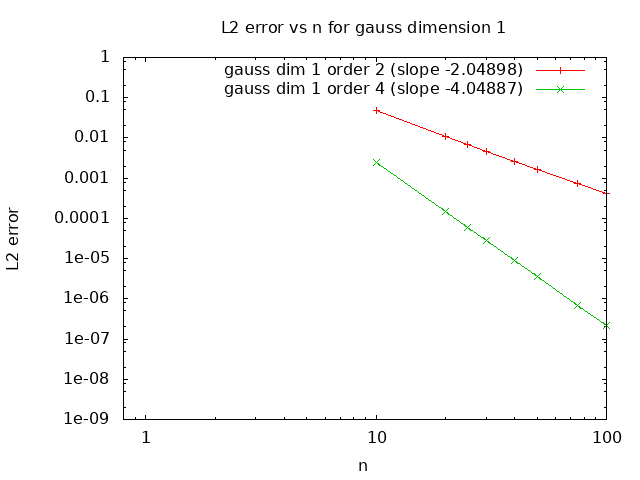
\includegraphics[width=.99\linewidth]{figures/convergence_gauss_dim1.png}
          \caption{1D}
          \label{fig:sub1}
        \end{subfigure}%
        \begin{subfigure}{.5\textwidth}
          \centering
          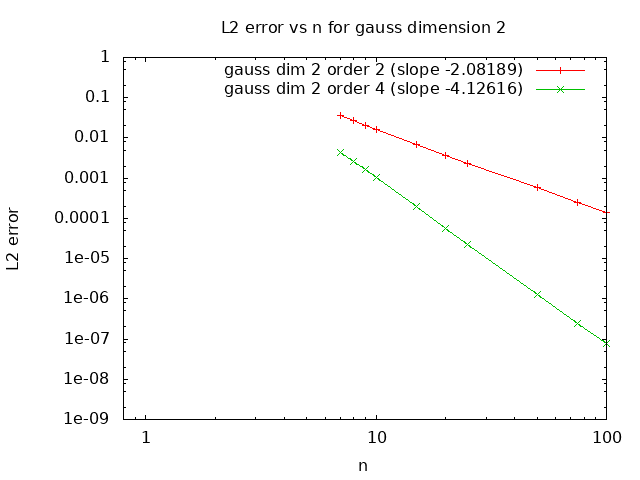
\includegraphics[width=.99\linewidth]{figures/convergence_gauss_dim2.png}
          \caption{2D}
          \label{fig:sub2}
        \end{subfigure}
        \caption{Convergence analysis of gauss-seidel solver}
        \label{fig:test}
        \end{figure}

        \item \underline{Jacobi solver}
        
        These are the grid convergence plots for the jacobi solver. We don't consider jacobi with 4th order solver since it is not stable. The expected slope was -2 for 2nd order. We have slopes pretty close to this expected value.
        
        \begin{figure}[H]
        \centering
        \begin{subfigure}{.5\textwidth}
          \centering
          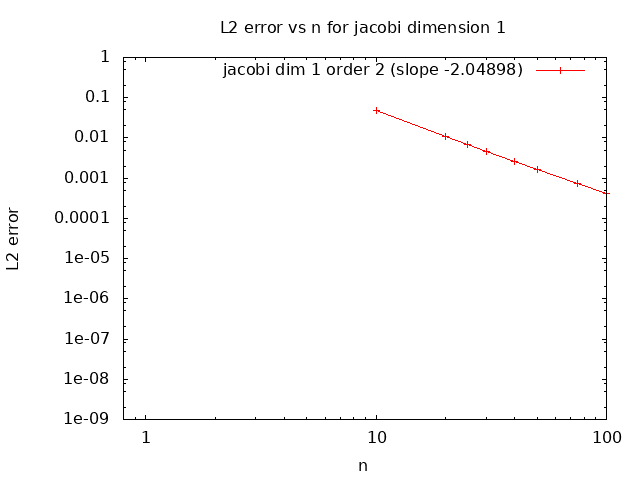
\includegraphics[width=.99\linewidth]{figures/convergence_jacobi_dim1.png}
          \caption{1D}
          \label{fig:sub1}
        \end{subfigure}%
        \begin{subfigure}{.5\textwidth}
          \centering
          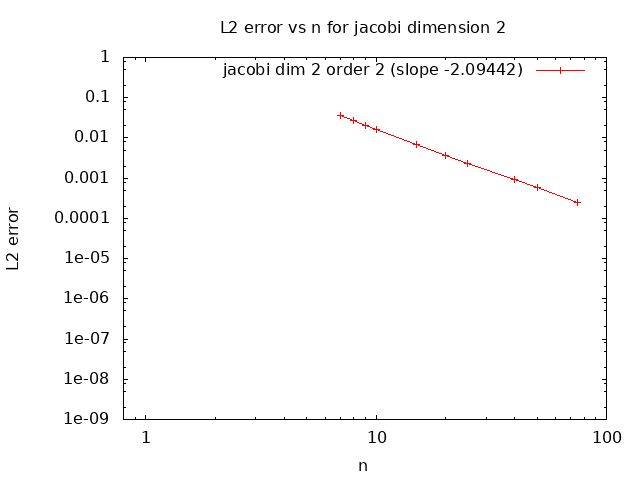
\includegraphics[width=.99\linewidth]{figures/convergence_jacobi_dim2.png}
          \caption{2D}
          \label{fig:sub2}
        \end{subfigure}
        \caption{Convergence analysis of jacobi solver}
        \label{fig:test}
        \end{figure}
    \end{itemize}
    Just for completeness, here we have two surface plots for a 4th order gauss 2D simulation on a \texttt{100x100} grid. Both plots look essentially similar.
  
          \begin{figure}[H]
        \centering
        \begin{subfigure}{.5\textwidth}
          \centering
          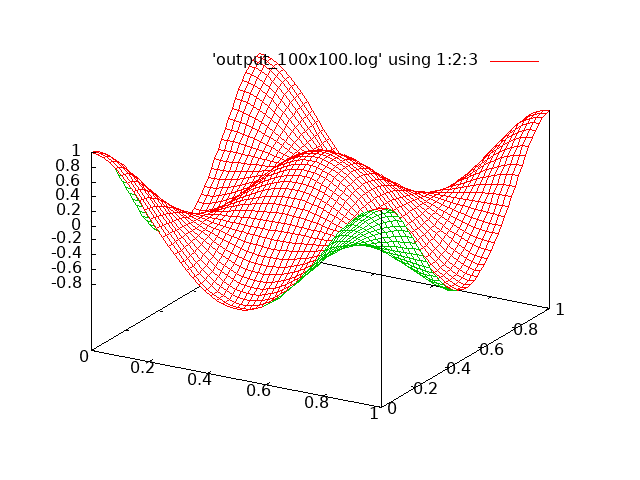
\includegraphics[width=.99\linewidth]{figures/surface_T_exact.png}
          \caption{T\_exact}
          \label{fig:sub1}
        \end{subfigure}%
        \begin{subfigure}{.5\textwidth}
          \centering
          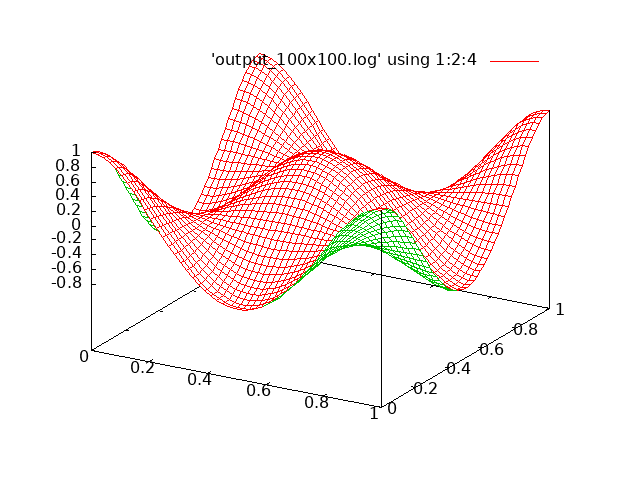
\includegraphics[width=.99\linewidth]{figures/surface_T_computed.png}
          \caption{T\_computed Gauss 4th order 100x100}
          \label{fig:sub2}
        \end{subfigure}
        \caption{Surface plots}
        \label{fig:test}
        \end{figure}

    \item \textbf{Runtime performance}
    
    A sample of time output for the given input configuration is shown below.
    \begin{lstlisting}[language=bash, basicstyle=\tiny]
--> verification_mode = 1
--> mode        = no_debug
--> n           = 20
--> dimension   = 2
--> length      = 1.000000
--> order       = 4
--> error_TOL   = 1.0000000000000001e-17
--> thermal_conductivity = 1.000000
--> max_iters   = 1000000
--> solver      = gauss

VERIFICATION MODE -
L2 norm of error for n 20   is   5.7410182758840052e-05

------------------------------------------------------------------------------------------------------------
GRVY Performance timing - Performance Timings:                       |      Mean      Variance       Count
--> gauss                            : 2.02494e-01 secs ( 94.6842 %) | [2.02494e-01  0.00000e+00          1]
--> write_results_output_file        : 4.57191e-03 secs (  2.1378 %) | [4.57191e-03  0.00000e+00          1]
--> q_order4_dim2                    : 1.84488e-03 secs (  0.8626 %) | [1.84488e-03  0.00000e+00          1]
--> main                             : 1.34730e-03 secs (  0.6300 %) | [1.34730e-03  0.00000e+00          1]
--> T_exact_order4_dim2              : 1.22809e-03 secs (  0.5742 %) | [1.22809e-03  0.00000e+00          1]
--> l2_norm                          : 9.53197e-04 secs (  0.4457 %) | [7.93670e-07  2.06032e-13       1201]
--> matrix_order4_dim2               : 7.10964e-04 secs (  0.3324 %) | [7.10964e-04  0.00000e+00          1]
--> print_matrix_A                   : 6.26087e-04 secs (  0.2928 %) | [6.26087e-04  0.00000e+00          1]
--> print_verification_mode          : 2.81334e-05 secs (  0.0132 %) | [2.81334e-05  0.00000e+00          1]
--> assemble_A                       : 5.00679e-06 secs (  0.0023 %) | [5.00679e-06  0.00000e+00          1]
--> print_vector_q                   : 3.09944e-06 secs (  0.0014 %) | [3.09944e-06  0.00000e+00          1]
--> print_compare_q_Texact_Tcomputed : 2.86102e-06 secs (  0.0013 %) | [2.86102e-06  0.00000e+00          1]
--> assemble_T_exact                 : 2.14577e-06 secs (  0.0010 %) | [2.14577e-06  0.00000e+00          1]
--> solve                            : 1.90735e-06 secs (  0.0009 %) | [1.90735e-06  0.00000e+00          1]
--> assemble_q                       : 9.53674e-07 secs (  0.0004 %) | [9.53674e-07  0.00000e+00          1]
--> GRVY_Unassigned                  : 4.19617e-05 secs (  0.0196 %)

                 Total Measured Time = 2.13863e-01 secs (100.0000 %)
------------------------------------------------------------------------------------------------------------
    \end{lstlisting}

The total time for various cases for various solver configurations is plotted and can be found below.

\begin{itemize}
    \item Gauss solver
            \begin{figure}[H]
        \centering
        \begin{subfigure}{.5\textwidth}
          \centering
          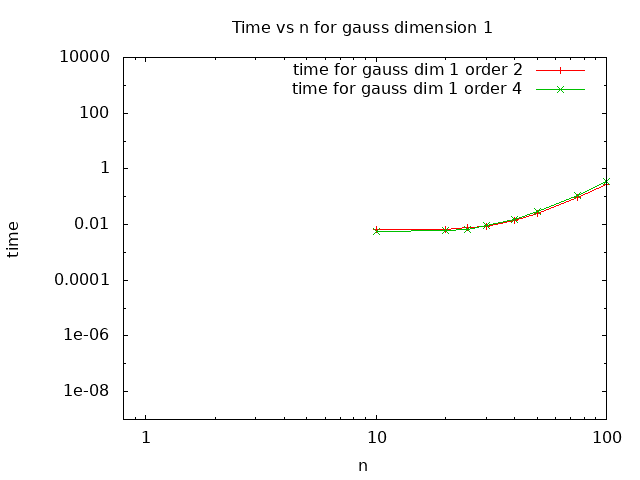
\includegraphics[width=.99\linewidth]{figures/time_gauss_dim1.png}
          \caption{1D}
          \label{fig:sub1}
        \end{subfigure}%
        \begin{subfigure}{.5\textwidth}
          \centering
          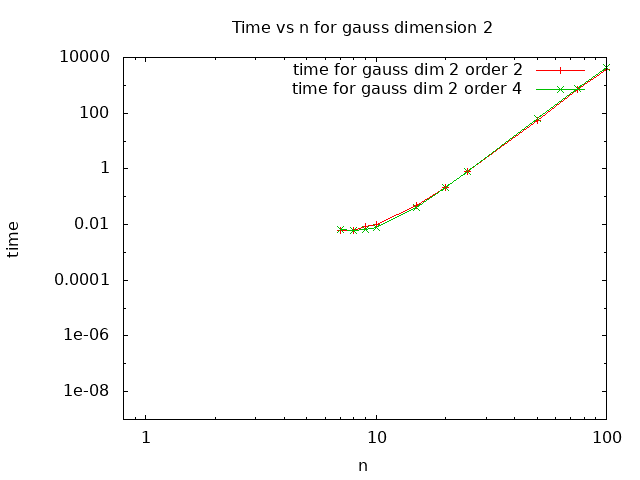
\includegraphics[width=.99\linewidth]{figures/time_gauss_dim2.png}
          \caption{2D}
          \label{fig:sub2}
        \end{subfigure}
        \caption{Runtime analysis of gauss solver}
        \label{fig:test}
        \end{figure}
    \item Jacobi
            \begin{figure}[H]
        \centering
        \begin{subfigure}{.5\textwidth}
          \centering
          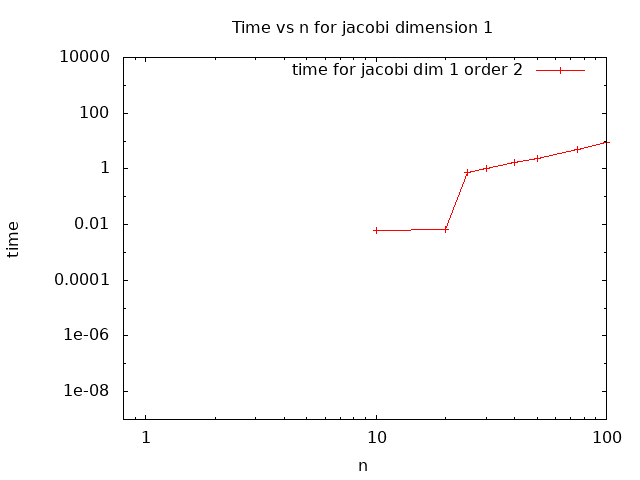
\includegraphics[width=.99\linewidth]{figures/time_jacobi_dim1.png}
          \caption{1D}
          \label{fig:sub1}
        \end{subfigure}%
        \begin{subfigure}{.5\textwidth}
          \centering
          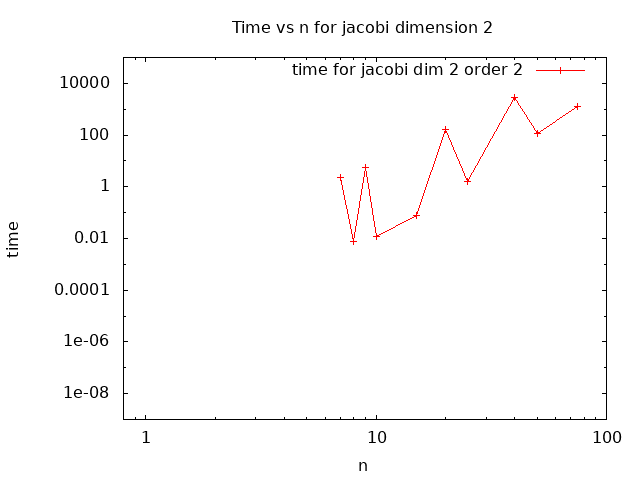
\includegraphics[width=.99\linewidth]{figures/time_jacobi_dim2.png}
          \caption{2D}
          \label{fig:sub2}
        \end{subfigure}
        \caption{Runtime analysis of jacobi solver}
        \label{fig:test}
        \end{figure}
\end{itemize}
\item \textbf{Regression testing}

\texttt{make check} runs the regression tests, which are stored in \texttt{proj02/tests/test.sh}. The sample output of \texttt{make check} is given below. (the colour is red due to \LaTeX but the test has actually passed). It shows only 1 test but technically the \texttt{test.sh} script contains 5 tests with the 4th test actually containing 4 tests and the 5th containing 2 tests. This makes a total of 9 tests.
\begin{lstlisting}[language=bash,basicstyle=\tiny]
Making check in src
make[1]: Entering directory `/home1/07665/shrey911/temp/cse380-2020-student-Shreyas911/proj02/src'
make[1]: Nothing to be done for `check'.
make[1]: Leaving directory `/home1/07665/shrey911/temp/cse380-2020-student-Shreyas911/proj02/src'
Making check in tests
make[1]: Entering directory `/home1/07665/shrey911/temp/cse380-2020-student-Shreyas911/proj02/tests'
make  check-TESTS
make[2]: Entering directory `/home1/07665/shrey911/temp/cse380-2020-student-Shreyas911/proj02/tests'
make[3]: Entering directory `/home1/07665/shrey911/temp/cse380-2020-student-Shreyas911/proj02/tests'
PASS: test.sh
make[4]: Entering directory `/home1/07665/shrey911/temp/cse380-2020-student-Shreyas911/proj02/tests'
make[4]: Nothing to be done for `all'.
make[4]: Leaving directory `/home1/07665/shrey911/temp/cse380-2020-student-Shreyas911/proj02/tests'
============================================================================
Testsuite summary for FULL-PACKAGE-NAME VERSION
============================================================================
# TOTAL: 1
# PASS:  1
# SKIP:  0
# XFAIL: 0
# FAIL:  0
# XPASS: 0
# ERROR: 0
============================================================================
make[3]: Leaving directory `/home1/07665/shrey911/temp/cse380-2020-student-Shreyas911/proj02/tests'
make[2]: Leaving directory `/home1/07665/shrey911/temp/cse380-2020-student-Shreyas911/proj02/tests'
make[1]: Leaving directory `/home1/07665/shrey911/temp/cse380-2020-student-Shreyas911/proj02/tests'
make[1]: Entering directory `/home1/07665/shrey911/temp/cse380-2020-student-Shreyas911/proj02'
make[1]: Leaving directory `/home1/07665/shrey911/temp/cse380-2020-student-Shreyas911/proj02'
\end{lstlisting}
Alternatively, you can run \texttt{proj02/tests/test.sh} directly, which gives the following output to \texttt{std::out}-


\begin{lstlisting}[language=bash,escapechar=\%]
$ ./test.sh 
%\checkmark% verify that the code is compiling
%\checkmark% verify that the verification mode runs fine
%\checkmark% verify that the debug mode runs fine
%\checkmark% verify all gauss solver outputs match reference outputs
%\checkmark% verify all jacobi solver outputs match reference outputs
\end{lstlisting}
\item \textbf{Code coverage}

Running \text{make coverage} as described above in the 'Running the primary code with petsc disabled and make coverage' section, we get a \texttt{proj02/coverage} directory. Tar it up, scp it to your local device, untar it and go inside to view \texttt{coverage/lcov/index.html}. You can find the \texttt{proj02/cover.tar.gz} tarball in the repo. You will see an output that looks as follows -

          \begin{figure}[H]
        \centering
          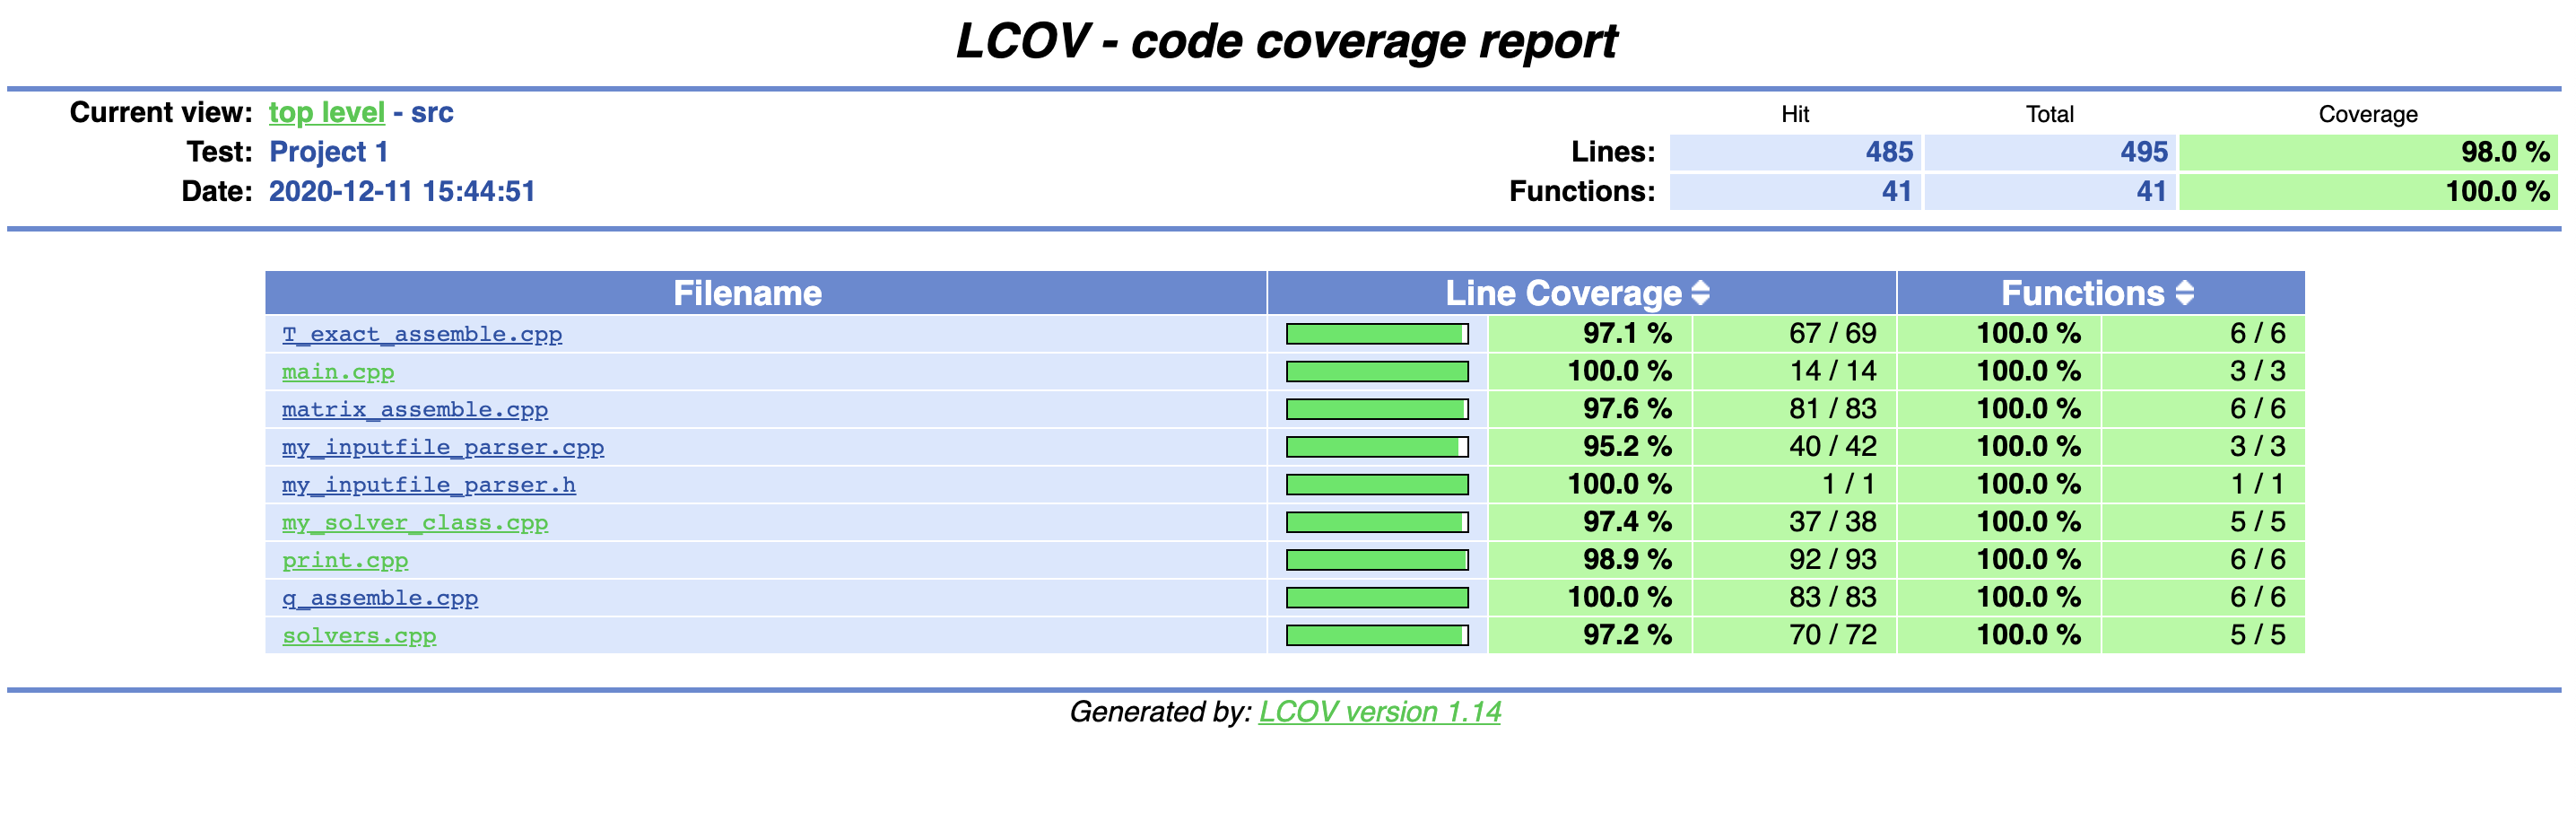
\includegraphics[width=.99\linewidth]{figures/lcov.png}
          \caption{lcov output}
        \label{fig:lcov}
        \end{figure}
\item \textbf{HDF5 I/O}
Shown below is a sample \texttt{.h5} file. We use \texttt{h5dump} for this purpose. The solver is jacobi and the rest of the metadata can be seen inside the \texttt{.h5} file itself.

\begin{lstlisting}[language=bash,escapechar=\%]
$ h5dump data.h5
HDF5 "data.h5" {
GROUP "/" {
   GROUP "coordinates" {
      DATASET "x data" {
         DATATYPE  H5T_IEEE_F64LE
         DATASPACE  SIMPLE { ( 100 ) / ( 100 ) }
         DATA {
         (0): 0, 0.111111, 0.222222, 0.333333, 0.444444, 0.555556, 0.666667,
         (7): 0.777778, 0.888889, 1, 0, 0.111111, 0.222222, 0.333333,
         (14): 0.444444, 0.555556, 0.666667, 0.777778, 0.888889, 1, 0,
         (21): 0.111111, 0.222222, 0.333333, 0.444444, 0.555556, 0.666667,
         (27): 0.777778, 0.888889, 1, 0, 0.111111, 0.222222, 0.333333,
         (34): 0.444444, 0.555556, 0.666667, 0.777778, 0.888889, 1, 0,
         (41): 0.111111, 0.222222, 0.333333, 0.444444, 0.555556, 0.666667,
         (47): 0.777778, 0.888889, 1, 0, 0.111111, 0.222222, 0.333333,
         (54): 0.444444, 0.555556, 0.666667, 0.777778, 0.888889, 1, 0,
         (61): 0.111111, 0.222222, 0.333333, 0.444444, 0.555556, 0.666667,
         (67): 0.777778, 0.888889, 1, 0, 0.111111, 0.222222, 0.333333,
         (74): 0.444444, 0.555556, 0.666667, 0.777778, 0.888889, 1, 0,
         (81): 0.111111, 0.222222, 0.333333, 0.444444, 0.555556, 0.666667,
         (87): 0.777778, 0.888889, 1, 0, 0.111111, 0.222222, 0.333333,
         (94): 0.444444, 0.555556, 0.666667, 0.777778, 0.888889, 1
         }
      }
      DATASET "y data" {
         DATATYPE  H5T_IEEE_F64LE
         DATASPACE  SIMPLE { ( 100 ) / ( 100 ) }
         DATA {
         (0): 0, 0, 0, 0, 0, 0, 0, 0, 0, 0, 0.111111, 0.111111, 0.111111,
         (13): 0.111111, 0.111111, 0.111111, 0.111111, 0.111111, 0.111111,
         (19): 0.111111, 0.222222, 0.222222, 0.222222, 0.222222, 0.222222,
         (25): 0.222222, 0.222222, 0.222222, 0.222222, 0.222222, 0.333333,
         (31): 0.333333, 0.333333, 0.333333, 0.333333, 0.333333, 0.333333,
         (37): 0.333333, 0.333333, 0.333333, 0.444444, 0.444444, 0.444444,
         (43): 0.444444, 0.444444, 0.444444, 0.444444, 0.444444, 0.444444,
         (49): 0.444444, 0.555556, 0.555556, 0.555556, 0.555556, 0.555556,
         (55): 0.555556, 0.555556, 0.555556, 0.555556, 0.555556, 0.666667,
         (61): 0.666667, 0.666667, 0.666667, 0.666667, 0.666667, 0.666667,
         (67): 0.666667, 0.666667, 0.666667, 0.777778, 0.777778, 0.777778,
         (73): 0.777778, 0.777778, 0.777778, 0.777778, 0.777778, 0.777778,
         (79): 0.777778, 0.888889, 0.888889, 0.888889, 0.888889, 0.888889,
         (85): 0.888889, 0.888889, 0.888889, 0.888889, 0.888889, 1, 1, 1, 1,
         (94): 1, 1, 1, 1, 1, 1
         }
      }
   }
   GROUP "metadata" {
      DATASET "dimensions" {
         DATATYPE  H5T_STD_I32LE
         DATASPACE  SIMPLE { ( 1 ) / ( 1 ) }
         DATA {
         (0): 2
         }
      }
      DATASET "grid_points" {
         DATATYPE  H5T_STD_I32LE
         DATASPACE  SIMPLE { ( 1 ) / ( 1 ) }
         DATA {
         (0): 10
         }
      }
      DATASET "order" {
         DATATYPE  H5T_STD_I32LE
         DATASPACE  SIMPLE { ( 1 ) / ( 1 ) }
         DATA {
         (0): 2
         }
      }
   }
   GROUP "temperature" {
      DATASET "Analytical Temperature" {
         DATATYPE  H5T_IEEE_F64LE
         DATASPACE  SIMPLE { ( 100 ) / ( 100 ) }
         DATA {
         (0): 1, 0.766044, 0.173648, -0.5, -0.939693, -0.939693, -0.5,
         (7): 0.173648, 0.766044, 1, 0.766044, 0.586824, 0.133022, -0.383022,
         (14): -0.719846, -0.719846, -0.383022, 0.133022, 0.586824, 0.766044,
         (20): 0.173648, 0.133022, 0.0301537, -0.0868241, -0.163176,
         (25): -0.163176, -0.0868241, 0.0301537, 0.133022, 0.173648, -0.5,
         (31): -0.383022, -0.0868241, 0.25, 0.469846, 0.469846, 0.25,
         (37): -0.0868241, -0.383022, -0.5, -0.939693, -0.719846, -0.163176,
         (43): 0.469846, 0.883022, 0.883022, 0.469846, -0.163176, -0.719846,
         (49): -0.939693, -0.939693, -0.719846, -0.163176, 0.469846,
         (54): 0.883022, 0.883022, 0.469846, -0.163176, -0.719846, -0.939693,
         (60): -0.5, -0.383022, -0.0868241, 0.25, 0.469846, 0.469846, 0.25,
         (67): -0.0868241, -0.383022, -0.5, 0.173648, 0.133022, 0.0301537,
         (73): -0.0868241, -0.163176, -0.163176, -0.0868241, 0.0301537,
         (78): 0.133022, 0.173648, 0.766044, 0.586824, 0.133022, -0.383022,
         (84): -0.719846, -0.719846, -0.383022, 0.133022, 0.586824, 0.766044,
         (90): 1, 0.766044, 0.173648, -0.5, -0.939693, -0.939693, -0.5,
         (97): 0.173648, 0.766044, 1
         }
      }
      DATASET "Numerical Temperature" {
         DATATYPE  H5T_IEEE_F64LE
         DATASPACE  SIMPLE { ( 100 ) / ( 100 ) }
         DATA {
         (0): 1, 0.766044, 0.173648, -0.5, -0.939693, -0.939693, -0.5,
         (7): 0.173648, 0.766044, 1, 0.766044, 0.594919, 0.137784, -0.384731,
         (14): -0.726125, -0.726125, -0.384731, 0.137784, 0.594919, 0.766044,
         (20): 0.173648, 0.137784, 0.0376302, -0.0772197, -0.152264,
         (25): -0.152264, -0.0772197, 0.0376302, 0.137784, 0.173648, -0.5,
         (31): -0.384731, -0.0772197, 0.27512, 0.505612, 0.505612, 0.27512,
         (37): -0.0772197, -0.384731, -0.5, -0.939693, -0.726125, -0.152264,
         (43): 0.505612, 0.935987, 0.935987, 0.505612, -0.152264, -0.726125,
         (49): -0.939693, -0.939693, -0.726125, -0.152264, 0.505612,
         (54): 0.935987, 0.935987, 0.505612, -0.152264, -0.726125, -0.939693,
         (60): -0.5, -0.384731, -0.0772197, 0.27512, 0.505612, 0.505612,
         (66): 0.27512, -0.0772197, -0.384731, -0.5, 0.173648, 0.137784,
         (72): 0.0376302, -0.0772197, -0.152264, -0.152264, -0.0772197,
         (77): 0.0376302, 0.137784, 0.173648, 0.766044, 0.594919, 0.137784,
         (83): -0.384731, -0.726125, -0.726125, -0.384731, 0.137784,
         (88): 0.594919, 0.766044, 1, 0.766044, 0.173648, -0.5, -0.939693,
         (95): -0.939693, -0.5, 0.173648, 0.766044, 1
         }
      }
   }
}
}


\end{lstlisting}
\item \textbf{Petsc solver}

Grid convergence as compared to gauss-seidel is shown in the plots below. We see that the error norms are almost identical to the gauss-seidel ones, thus completing our verification for petsc. For 2D, petsc was run up to n=50 due to lack of time.

       \begin{figure}[H]
        \centering
        \begin{subfigure}{.5\textwidth}
          \centering
          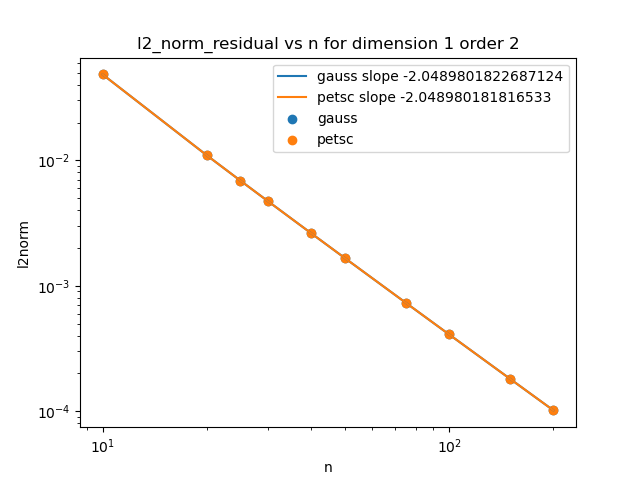
\includegraphics[width=.99\linewidth]{figures/l2norm_petsc_gauss_order_2_dimension_1.png}
          \caption{1D}
          \label{fig:sub1}
        \end{subfigure}%
        \begin{subfigure}{.5\textwidth}
          \centering
          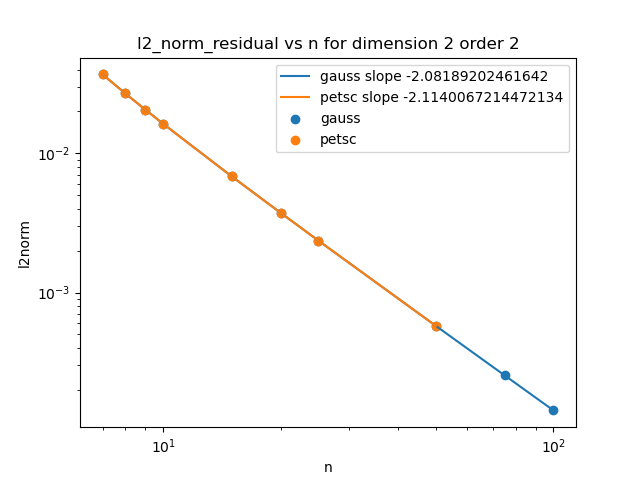
\includegraphics[width=.99\linewidth]{figures/l2norm_petsc_gauss_order_2_dimension_2.png}
          \caption{2D}
          \label{fig:sub2}
        \end{subfigure}
        \caption{Convergence analysis of petsc solver for order 2}
        \label{fig:test}
        \end{figure}
       \begin{figure}[H]
        \centering
        \begin{subfigure}{.5\textwidth}
          \centering
          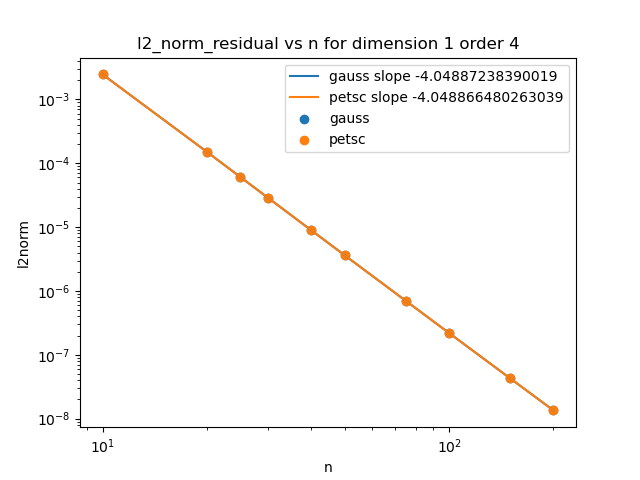
\includegraphics[width=.99\linewidth]{figures/l2norm_petsc_gauss_order_4_dimension_1.png}
          \caption{1D}
          \label{fig:sub1}
        \end{subfigure}%
        \begin{subfigure}{.5\textwidth}
          \centering
          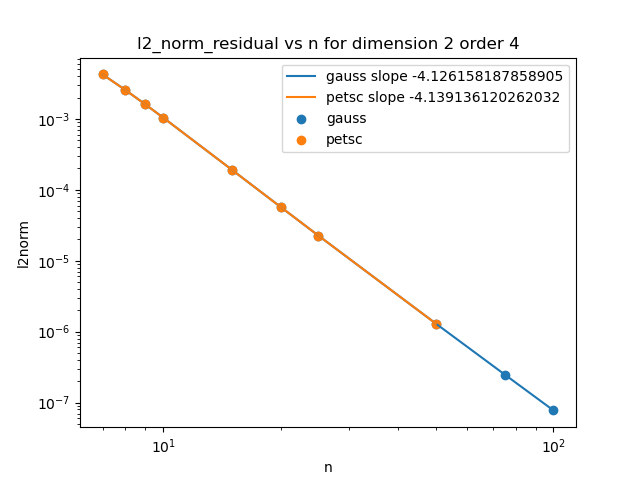
\includegraphics[width=.99\linewidth]{figures/l2norm_petsc_gauss_order_4_dimension_2.png}
          \caption{2D}
          \label{fig:sub2}
        \end{subfigure}
        \caption{Convergence analysis of petsc solver for order 4}
        \label{fig:test}
        \end{figure}
        
Next we have the timing comparison plots of all three solvers. petsc does well for 1D compared to other solvers, but not so well for 2D (meaning petsc does badly for super large number of points). This might be because the whole pipeline is not set up for petsc, for example assembling was done without inbuilt functions from petsc. 

       \begin{figure}[H]
        \centering
        \begin{subfigure}{.5\textwidth}
          \centering
          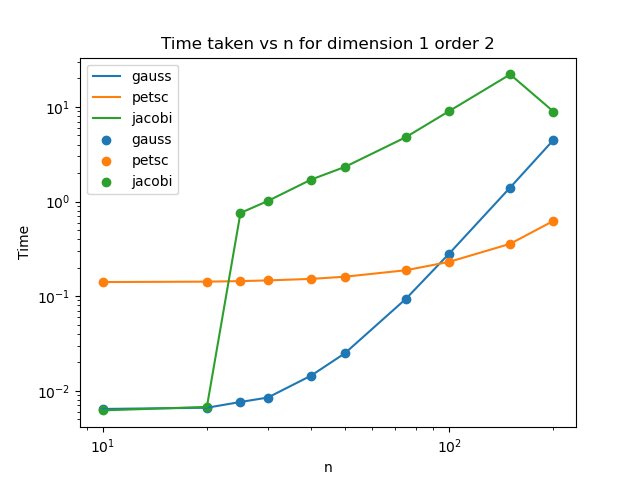
\includegraphics[width=.99\linewidth]{figures/time_all_solvers_order_2_dimension_1.png}
          \caption{1D}
          \label{fig:sub1}
        \end{subfigure}%
        \begin{subfigure}{.5\textwidth}
          \centering
          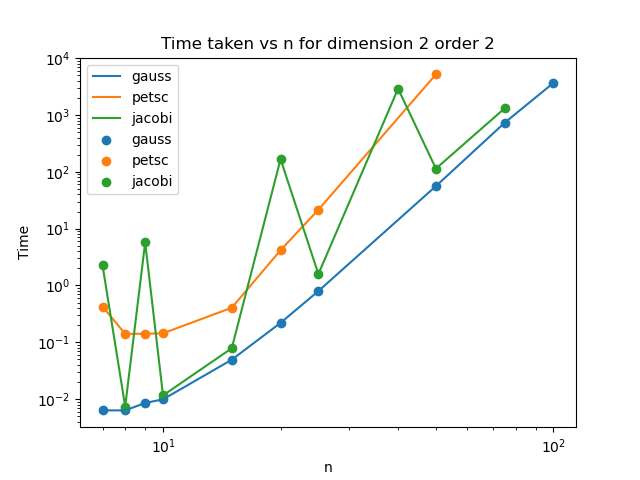
\includegraphics[width=.99\linewidth]{figures/time_all_solvers_order_2_dimension_2.png}
          \caption{2D}
          \label{fig:sub2}
        \end{subfigure}
        \caption{Timing comparison of all solvers for order 2}
        \label{fig:test}
        \end{figure}
        
       \begin{figure}[H]
        \centering
        \begin{subfigure}{.5\textwidth}
          \centering
          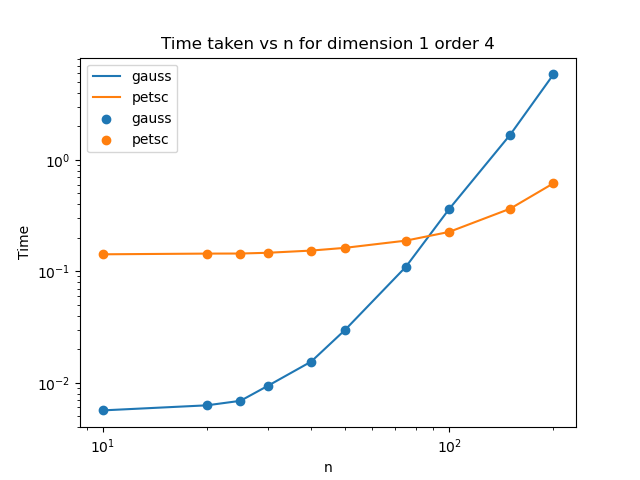
\includegraphics[width=.99\linewidth]{figures/time_all_solvers_order_4_dimension_1.png}
          \caption{1D}
          \label{fig:sub1}
        \end{subfigure}%
        \begin{subfigure}{.5\textwidth}
          \centering
          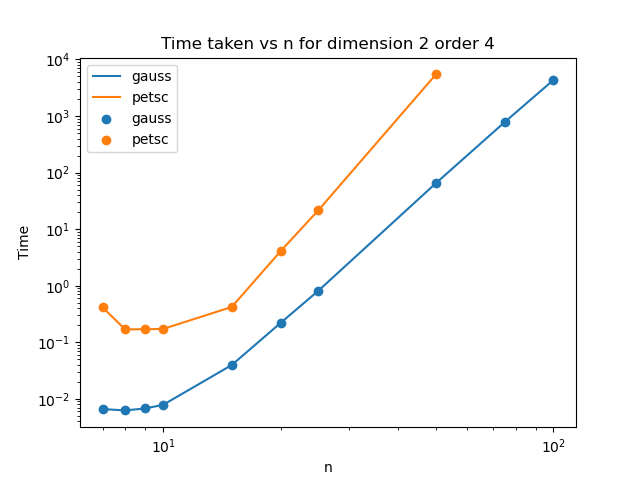
\includegraphics[width=.99\linewidth]{figures/time_all_solvers_order_4_dimension_2.png}
          \caption{2D}
          \label{fig:sub2}
        \end{subfigure}
        \caption{Timing comparison of gauss and petsc solvers for order 4}
        \label{fig:test}
        \end{figure}

\item \textbf{Beautiful plots using hdf5 files}

We use \texttt{h5py} for this purpose. The plotting script is \texttt{h5py\_surface\_plotter.py}.

          \begin{figure}[H]
        \centering
        \begin{subfigure}{.5\textwidth}
          \centering
          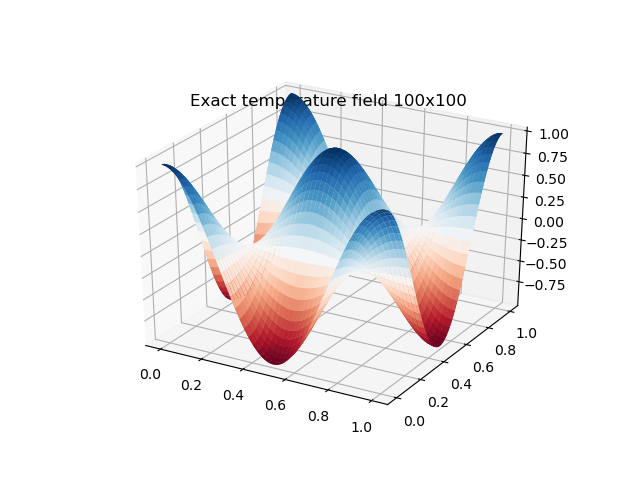
\includegraphics[width=.99\linewidth]{figures/hdf5_surface_exact_plot.png}
          \caption{T\_exact}
          \label{fig:sub1}
        \end{subfigure}%
        \begin{subfigure}{.5\textwidth}
          \centering
          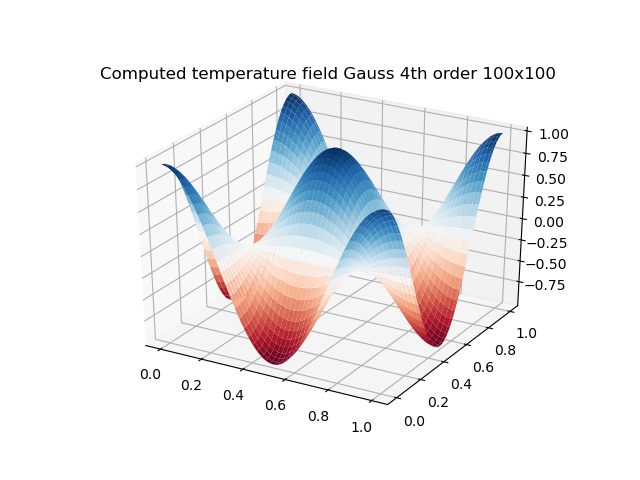
\includegraphics[width=.99\linewidth]{figures/hdf5_surface_computed_plot.png}
          \caption{T\_computed Gauss 4th order 100x100}
          \label{fig:sub2}
        \end{subfigure}
        \caption{Surface plots}
        \label{fig:test}
        \end{figure}
        
                  \begin{figure}[H]
        \centering
        \begin{subfigure}{.5\textwidth}
          \centering
          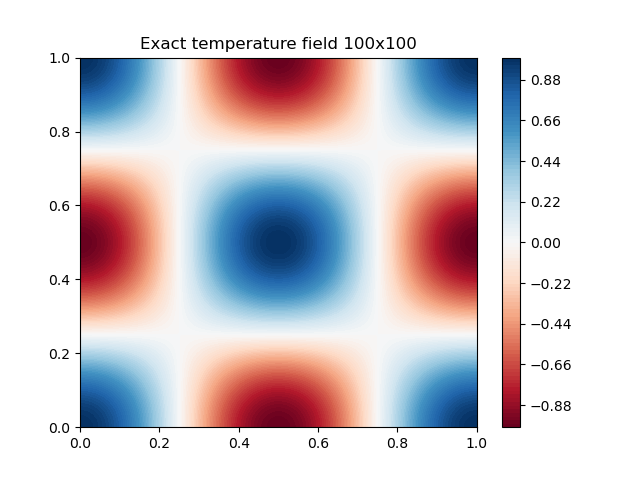
\includegraphics[width=.99\linewidth]{figures/hdf5_contourf_exact_plot.png}
          \caption{T\_exact}
          \label{fig:sub1}
        \end{subfigure}%
        \begin{subfigure}{.5\textwidth}
          \centering
          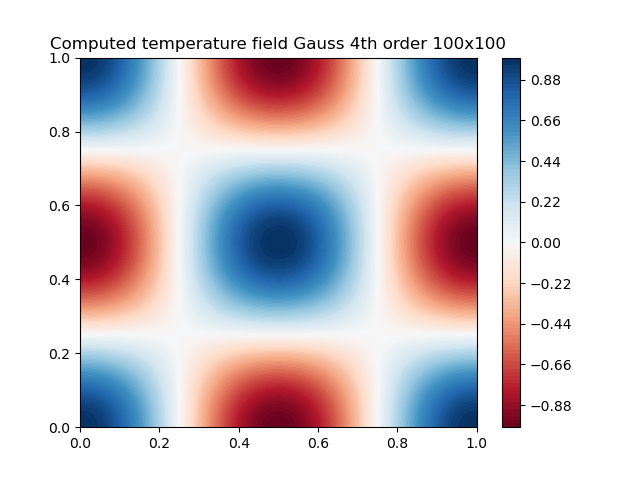
\includegraphics[width=.99\linewidth]{figures/hdf5_contourf_computed_plot.png}
          \caption{T\_computed Gauss 4th order 100x100}
          \label{fig:sub2}
        \end{subfigure}
        \caption{Contour filled plots}
        \label{fig:test}
        \end{figure}

\item \textbf{Continuous integration}

The dockerfile used for the container can be found in \texttt{proj02/src/}. The only difference between Karl's file and mine is that I have also installed vim. Here is the dockerfile for convenience.
\begin{lstlisting}[language=bash,escapechar=\%]
FROM centos:7
MAINTAINER Karl W. Schulz <karl@oden.utexas.edu>

# Define a user
RUN useradd -u 2000 -m test

# enable OpenHPC repository
RUN yum install -y https://github.com/openhpc/ohpc/releases/download/v1.3.GA/ohpc-release-1.3-1.el7.x86_64.rpm

# Add some packages
RUN yum -y install make which git
RUN yum -y install vim
RUN yum -y install ohpc-autotools
RUN yum -y install valgrind-ohpc
RUN yum -y install gnu8-compilers-ohpc
RUN yum -y install gsl-gnu8-ohpc hdf5-gnu8-ohpc
RUN yum -y install openmpi3-gnu8-ohpc boost-gnu8-openmpi3-ohpc petsc-gnu8-openmpi3-ohpc
RUN yum -y install lmod-defaults-gnu8-openmpi3-ohpc
RUN yum -y install bc wget zlib-devel perl-Digest-MD5
# Add Bats
RUN yum -y install bats
# Add MASA
ENV masa_ver=0.50.0
RUN wget https://github.com/manufactured-solutions/MASA/releases/download/$masa_ver/masa-$masa_ver.tar.gz -P /tmp
RUN cd /tmp; tar xfz /tmp/masa-$masa_ver.tar.gz
RUN . /etc/profile.d/lmod.sh \
    && cd /tmp/masa-$masa_ver \
    && ./configure --enable-fortran-interfaces \
    && make \
    && make install
RUN rm /tmp/masa-$masa_ver.tar.gz
# Add GRVY
ENV grvy_ver="0.34.0"
RUN wget https://github.com/hpcsi/grvy/releases/download/$grvy_ver/grvy-$grvy_ver.tar.gz -P /tmp
RUN cd /tmp; tar xfz /tmp/grvy-$grvy_ver.tar.gz
RUN . /etc/profile.d/lmod.sh \
    && module load boost \
    && cd /tmp/grvy-$grvy_ver \
    && ./configure CXXFLAGS="-std=c++11" LDFLAGS="-Wl,-rpath,$BOOST_LIB" \
    && make \
    && make install
RUN rm /tmp/grvy-$grvy_ver.tar.gz

# Register new libs installed into /usr/local/lib with linker
RUN echo "/usr/local/lib" > /etc/ld.so.conf.d/class.conf
RUN ldconfig

# User to run as
WORKDIR /home/test
USER test
\end{lstlisting}

Here is the \texttt{.travis.yml} file for reference. The configure command is much simpler inside the docker as you can see.

\begin{lstlisting}[language=bash,escapechar=\%]
sudo: required
language: C

services:
        - docker

before_install:
        - docker pull shreyas911/my_docker_image:v1.0
        - export DOCKER_RUN="docker run -v ${TRAVIS_BUILD_DIR}:/home/test/ shreyas911/my_docker_image:v1.0"

script:
        - ${DOCKER_RUN} /bin/bash -l -c "module load petsc && cd proj02 && autoreconf -f -i && ./configure CC=mpicc CXX=mpicxx --enable-coverage && make && make check"

notifications:
        email: false
\end{lstlisting}
The Travis CI tests complete successfully, a screenshot of the sample output is given below. The build is \#36 on travis.

          \begin{figure}[H]
        \centering
          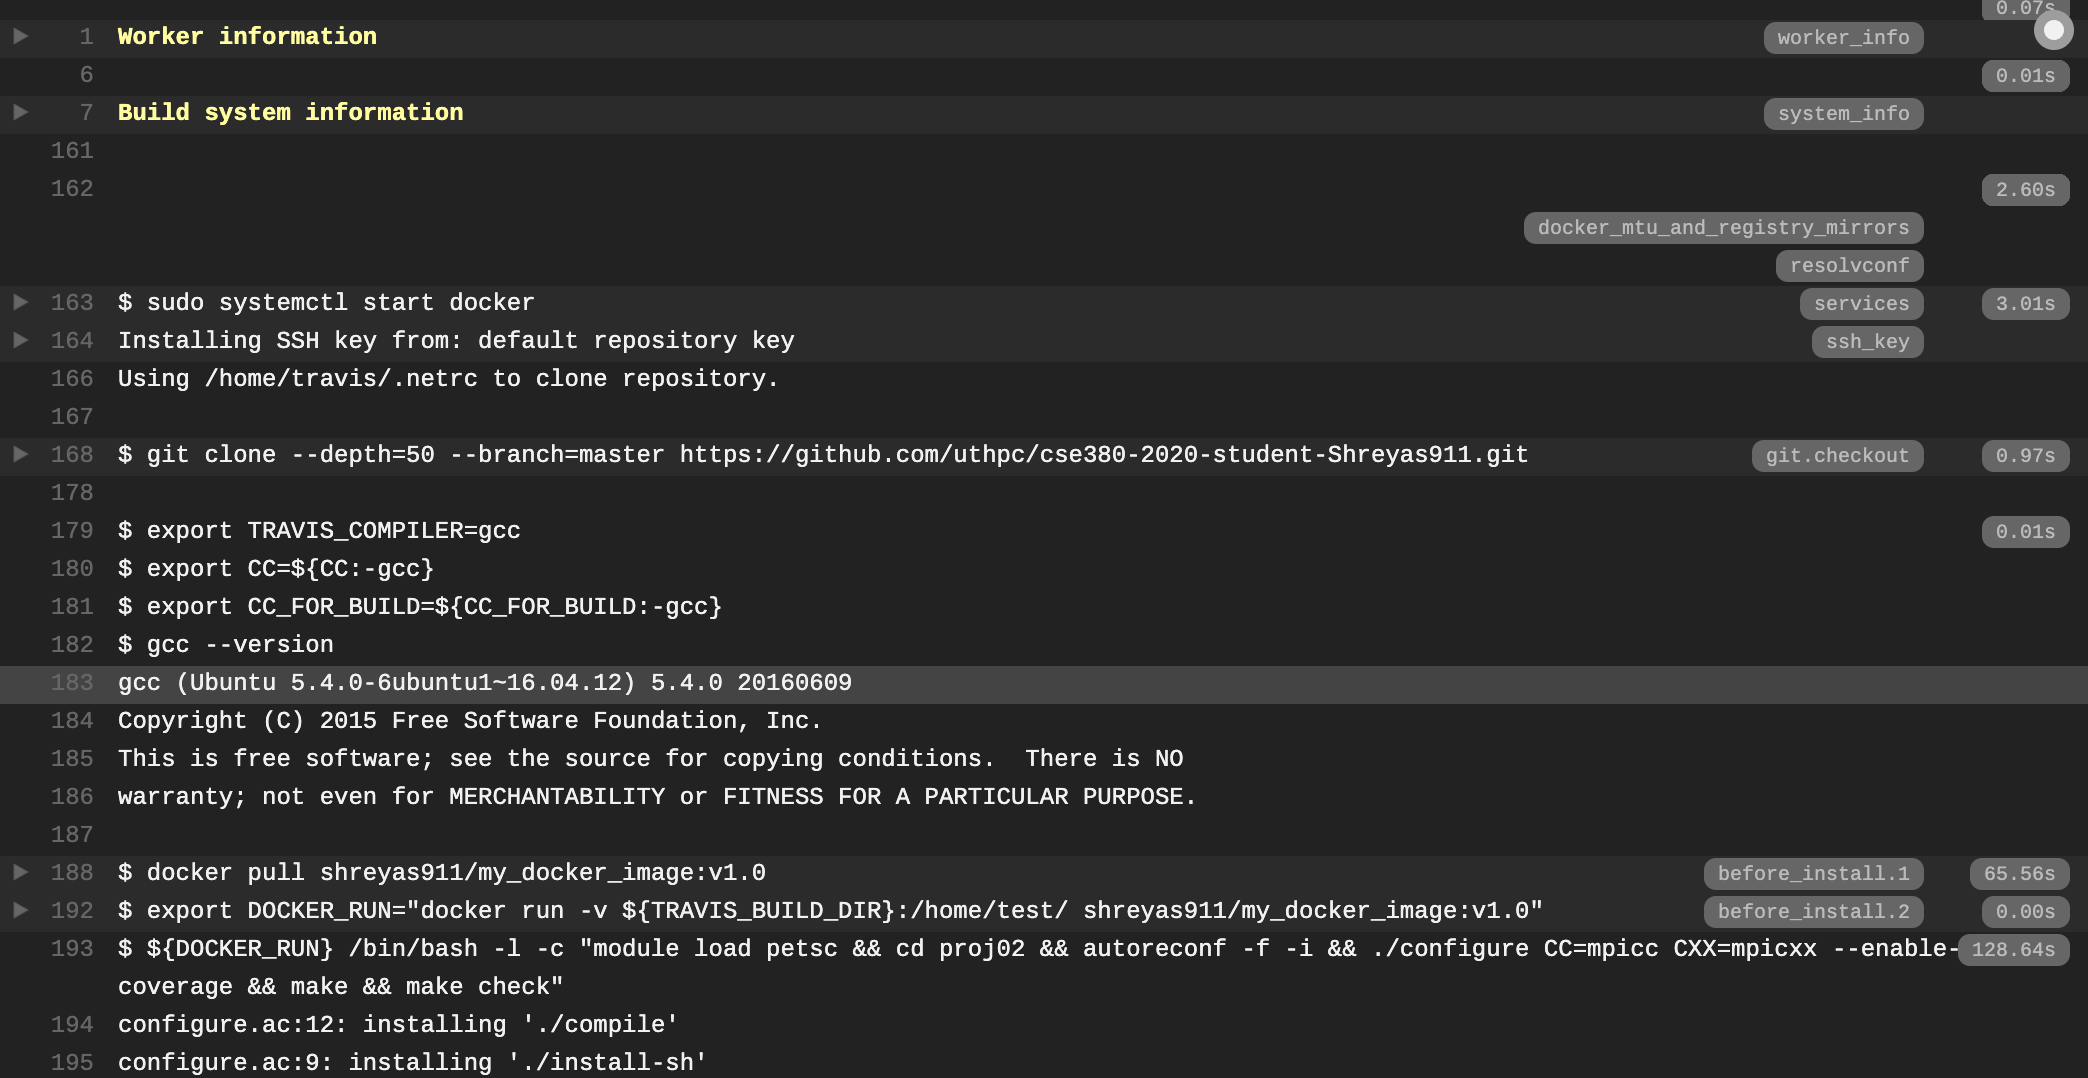
\includegraphics[width=.99\linewidth]{figures/travis1.png}

        \label{fig:travis}
        \end{figure}
                  \begin{figure}[H]
        \centering
          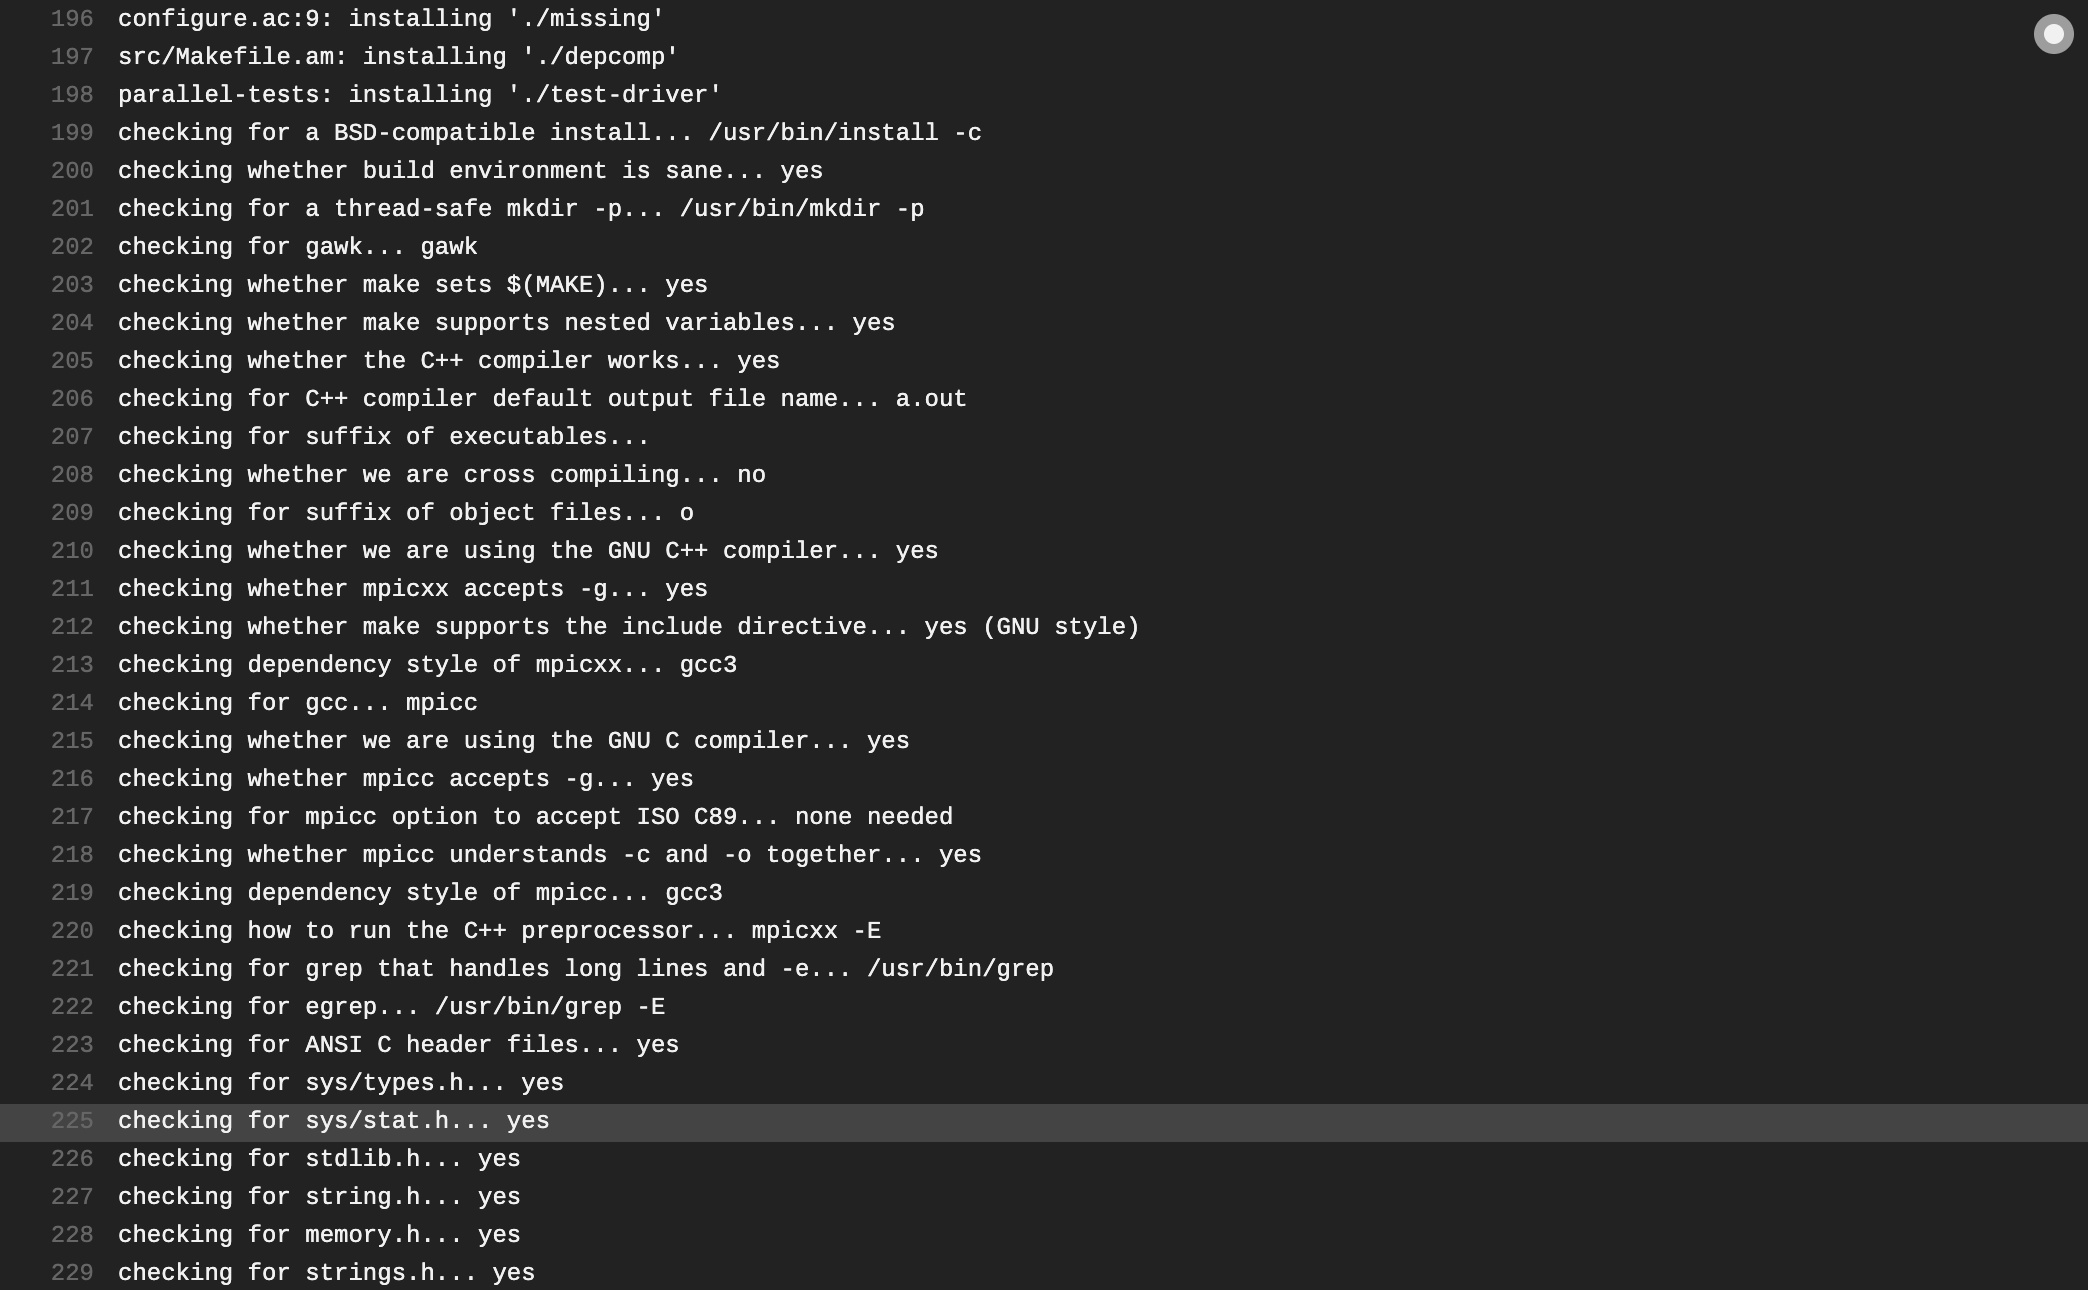
\includegraphics[width=.99\linewidth]{figures/travis2.png}

        \label{fig:travis}
        \end{figure}
                  \begin{figure}[H]
        \centering
          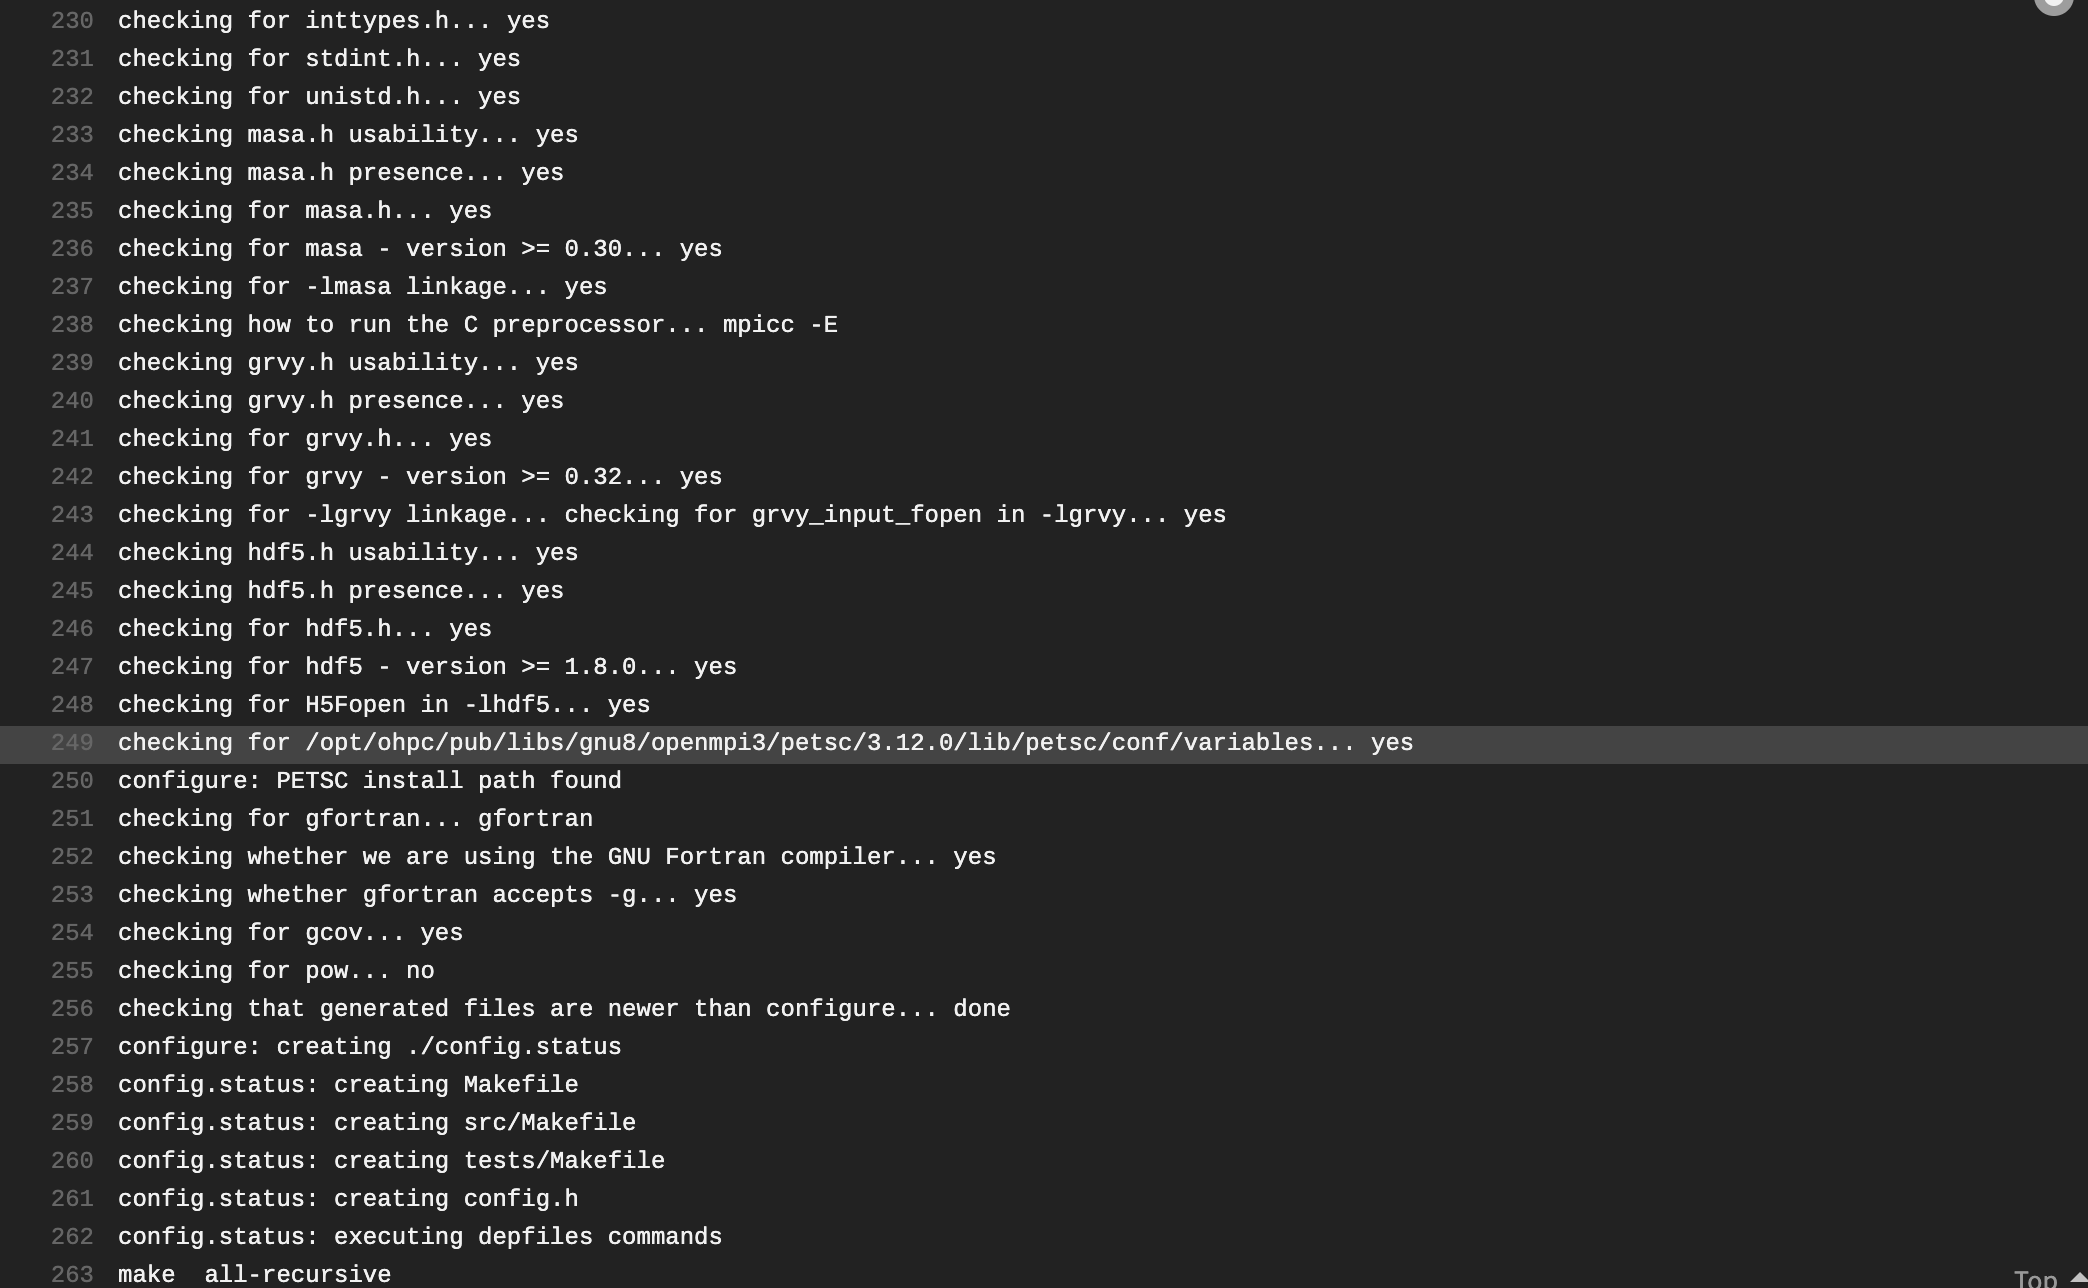
\includegraphics[width=.99\linewidth]{figures/travis3.png}

        \label{fig:travis}
        \end{figure}
                  \begin{figure}[H]
        \centering
          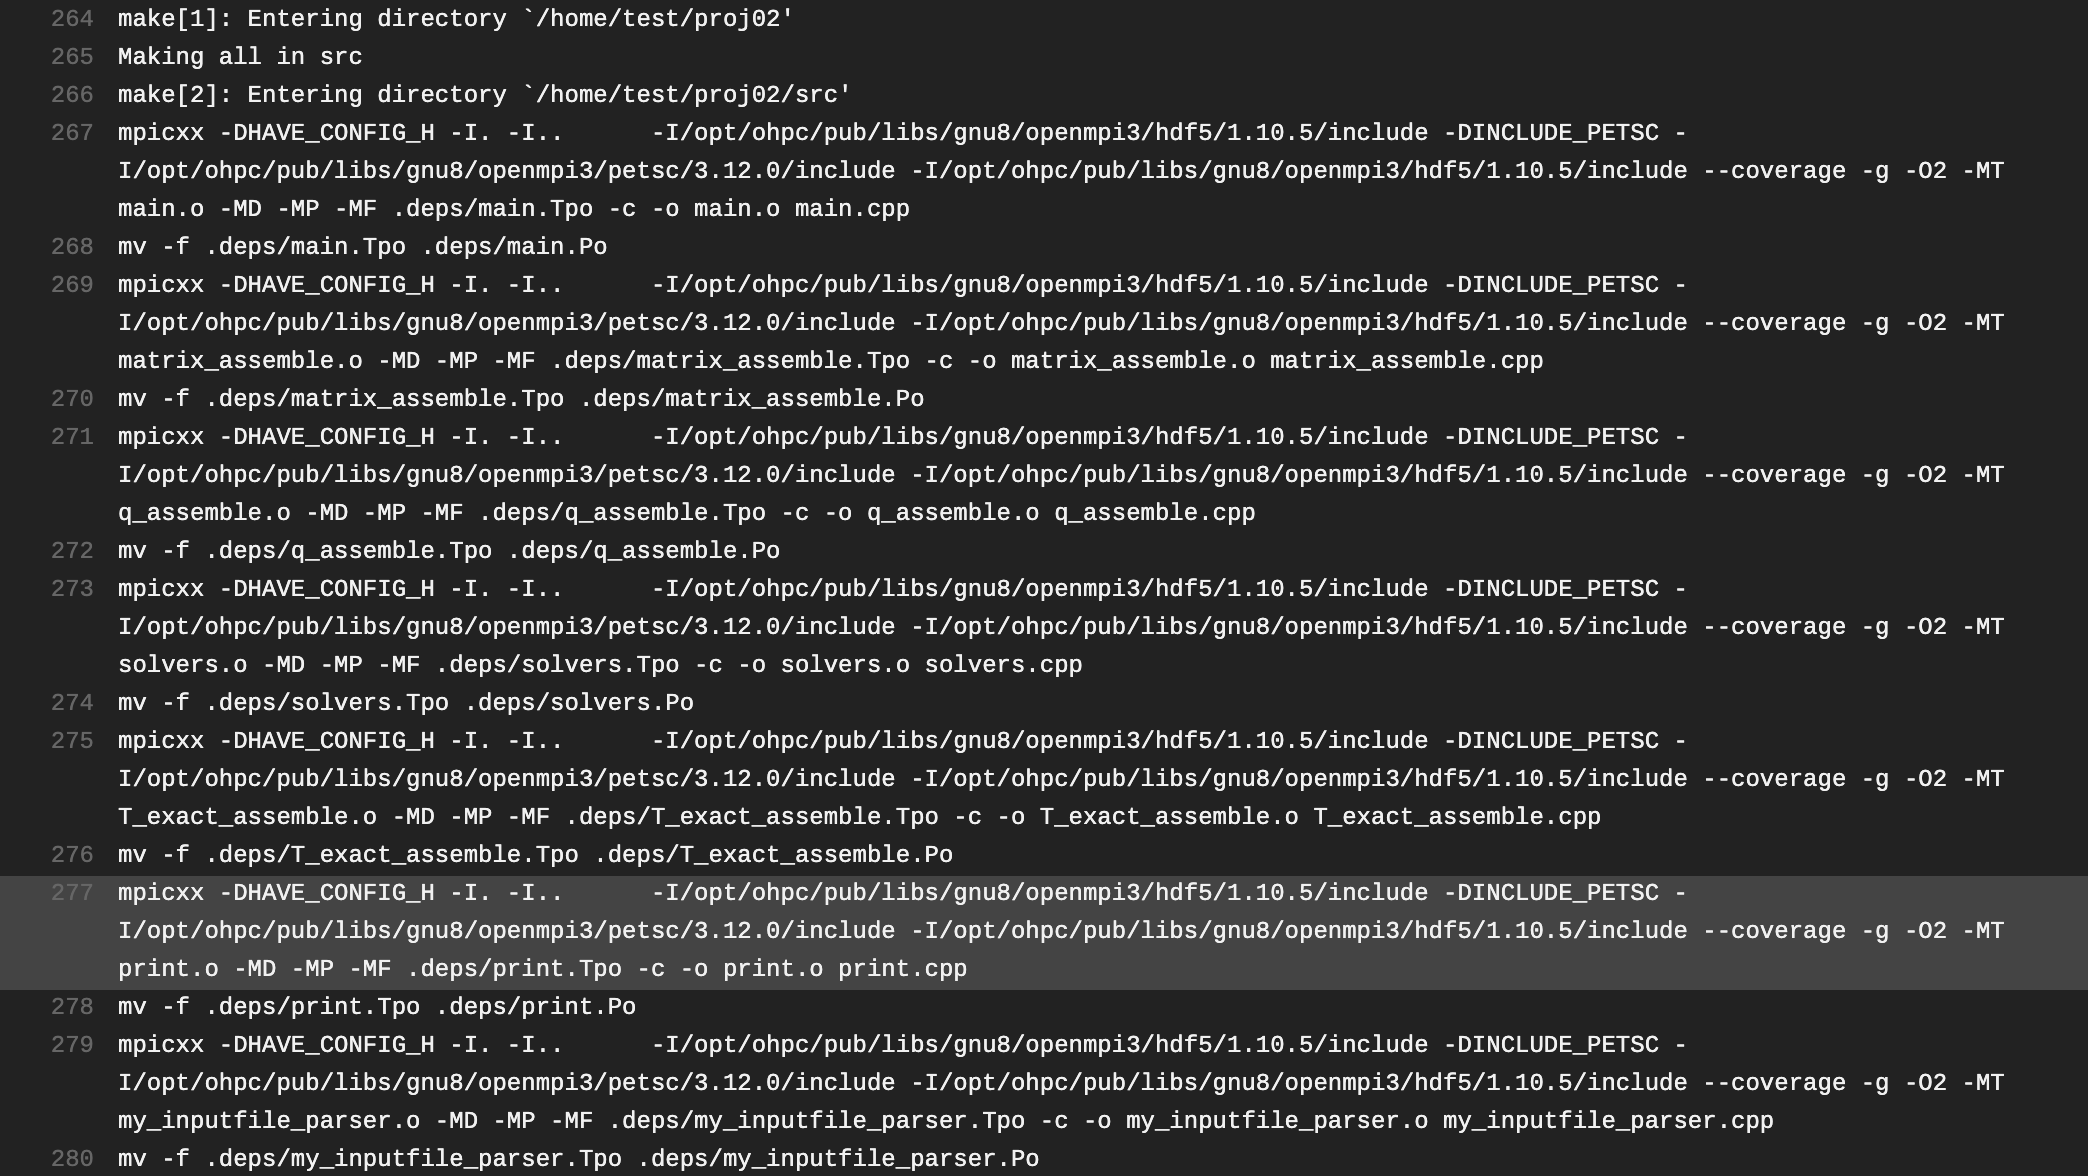
\includegraphics[width=.99\linewidth]{figures/travis4.png}

        \label{fig:travis}
        \end{figure}
                  \begin{figure}[H]
        \centering
          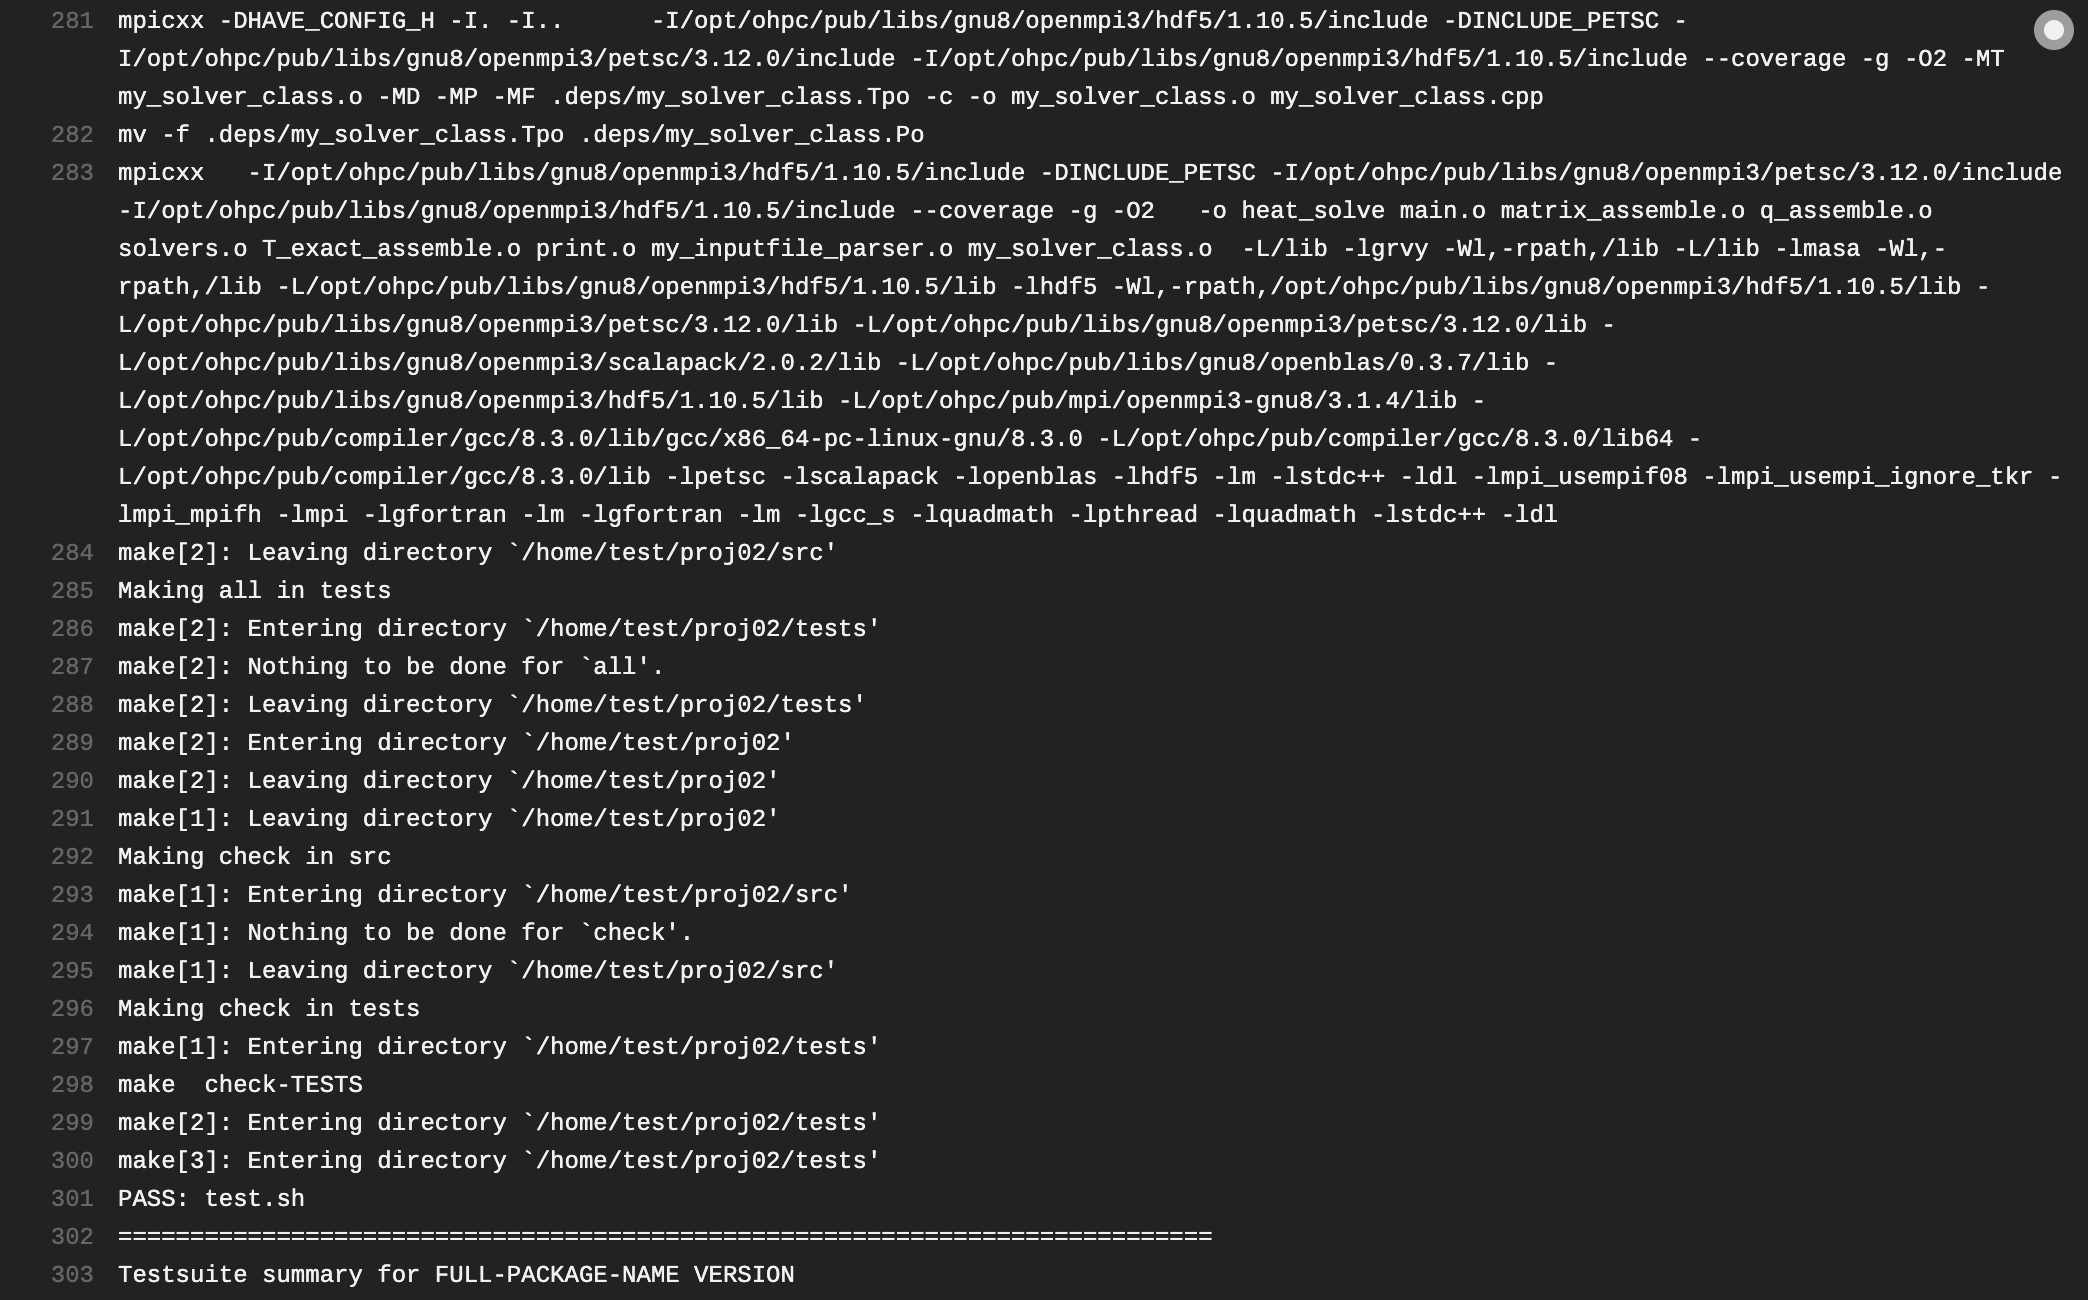
\includegraphics[width=.99\linewidth]{figures/travis5.png}

        \label{fig:travis}
        \end{figure}
                  \begin{figure}[H]
        \centering
          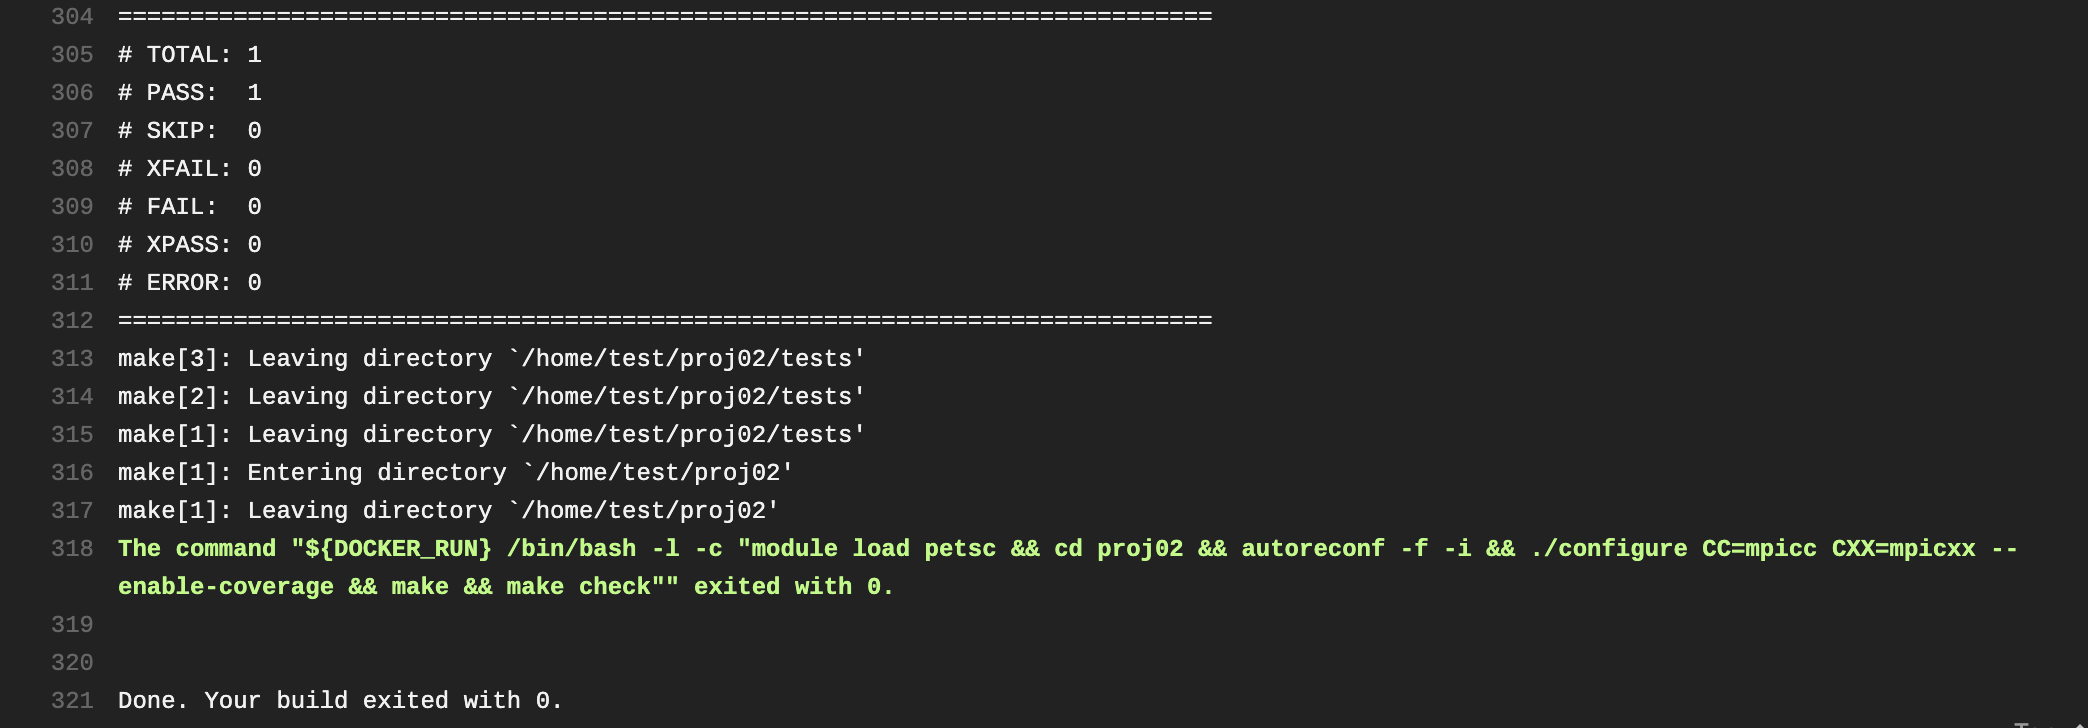
\includegraphics[width=.99\linewidth]{figures/travis6.png}
          \caption{Travis output}
        \label{fig:travis}
        \end{figure}
\end{itemize}

% \appendix
% \section{Sparsity patterns}\label{A}
% \subsection{2D Second order approximation}\label{A.1}
%         The sparsity pattern of $\mathbf{A_x}$ is given by, (illustration for a $5\times5$ grid)
%          \begin{align*}
%                 \mathbf{A_x} &= \left[\begin{smallmatrix} 
%                 \\
%                 & \\
%                 && \\
%                 &&& \\
%                 &&&& \\
%                 &&&&& \\
%                 &&&&& \d & \d & \d\\
%                 &&&&&& \d & \d & \d\\
%                 &&&&&&& \d & \d & \d\\
%                 &&&&&&&& \\
%                 &&&&&&&&& \\
%                 &&&&&&&&&& \d & \d & \d\\ 
%                 &&&&&&&&&&& \d & \d & \d\\
%                 &&&&&&&&&&&& \d & \d & \d\\
%                 &&&&&&&&&&&& \\
%                 &&&&&&&&&&&&& \\
%                 &&&&&&&&&&&&&&& \d & \d & \d\\
%                 &&&&&&&&&&&&&&&& \d & \d & \d\\
%                 &&&&&&&&&&&&&&&&& \d & \d & \d\\
%                 &&&&&&&&&&&&&&&&&&& \\
%                 &&&&&&&&&&&&&&&&&&&& \\
%                 &&&&&&&&&&&&&&&&&&&&& \\
%                 &&&&&&&&&&&&&&&&&&&&&& \\
%                 &&&&&&&&&&&&&&&&&&&&&&& \\
%                 &&&&&&&&&&&&&&&&&&&&&&&& \\
%                 \end{smallmatrix}\right]
%             \end{align*}
%             The sparsity pattern of $\mathbf{A_y}$ is given by, (illustration for a $5\times5$ grid) 
%             \begin{align*}
%                 \mathbf{A_y} &= \left[\begin{smallmatrix} 
%                 \\
%                 & \\
%                 && \\
%                 &&& \\
%                 &&&& \\
%                 &&&&& \\
%                 & \d &&&&& \d &&&&& \d\\
%                 && \d &&&&& \d &&&&& \d\\
%                 &&& \d &&&&& \d &&&&& \d\\
%                 &&&&&&&&& \\
%                 &&&&&&&&&& \\
%                 &&&&&&& \d &&&&& \d &&&&& \d\\
%                 &&&&&&&& \d &&&&& \d &&&&& \d\\
%                 &&&&&&&&& \d &&&&& \d &&&&& \d\\
%                 &&&&&&&&&&&&&& \\
%                 &&&&&&&&&&&&&&& \\
%                 &&&&&&&&&&&&& \d &&&&& \d &&&&& \d\\
%                 &&&&&&&&&&&&&& \d &&&&& \d &&&&& \d\\
%                 &&&&&&&&&&&&&&& \d &&&&& \d &&&&& \d\\
%                 &&&&&&&&&&&&&&&&&&&&& \\
%                 &&&&&&&&&&&&&&&&&&&&&& \\
%                 &&&&&&&&&&&&&&&&&&&&&&& \\
%                 &&&&&&&&&&&&&&&&&&&&&&&& \\
%                 &&&&&&&&&&&&&&&&&&&&&&&&& \\
%                 &&&&&&&&&&&&&&&&&&&&&&&&&& \\
%                 \end{smallmatrix}\right]
%             \end{align*}            
%             The sparsity pattern of $\mathbf{A_b}$ is given by, (illustration for a $5\times5$ grid) 
%             \begin{align*}
%                 \mathbf{A_b} &= \left[\begin{smallmatrix} 
%                 \d\\
%                 & \d\\
%                 && \d\\
%                 &&& \d\\
%                 &&&& \d\\
%                 &&&&& \d\\
%                 &&&&&& \\
%                 &&&&&&& \\
%                 &&&&&&&& \\
%                 &&&&&&&&& \d\\
%                 &&&&&&&&&& \d\\
%                 &&&&&&&&&&& \\
%                 &&&&&&&&&&&& \\
%                 &&&&&&&&&&&&& \\
%                 &&&&&&&&&&&&&& \d\\
%                 &&&&&&&&&&&&&&& \d\\
%                 &&&&&&&&&&&&&&&& \\
%                 &&&&&&&&&&&&&&&&& \\
%                 &&&&&&&&&&&&&&&&&& \\
%                 &&&&&&&&&&&&&&&&&&& \d\\
%                 &&&&&&&&&&&&&&&&&&&& \d\\
%                 &&&&&&&&&&&&&&&&&&&&& \d\\
%                 &&&&&&&&&&&&&&&&&&&&&& \d\\
%                 &&&&&&&&&&&&&&&&&&&&&&& \d\\
%                 &&&&&&&&&&&&&&&&&&&&&&&& \d\\
%                 \end{smallmatrix}\right]
%             \end{align*}
% \subsection{2D Fourth order approximation}\label{A.2}

%             The sparsity pattern of $\mathbf{A_x}$ is given by, (illustration for a $7\times7$ grid)
%             \begin{align*}
%                 \mathbf{A_x} &= \left[\begin{smallmatrix} 
%                 \\
%                 & \\
%                 && \\
%                 &&& \\
%                 &&&& \\
%                 &&&&& \\
%                 &&&&&& \\
%                 &&&&&& \\
%                 &&&&&& \d & \d & \d & \d & \d\\
%                 &&&&&&& \d & \d & \d & \d & \d\\
%                 &&&&&&&& \d & \d & \d & \d & \d\\
%                 &&&&&&&&& \\
%                 &&&&&&&&&&& \\
%                 &&&&&&&&&&&& \\ 
%                 &&&&&&&&&&&& \\
%                 &&&&&&&&&&&&& \d & \d & \d & \d & \d\\
%                 &&&&&&&&&&&&&& \d & \d & \d & \d & \d\\
%                 &&&&&&&&&&&&&&& \d & \d & \d & \d & \d\\
%                 &&&&&&&&&&&&&&& \\
%                 &&&&&&&&&&&&&&&& \\
%                 &&&&&&&&&&&&&&&&& \\ 
%                 &&&&&&&&&&&&&&&&&& \\
%                 &&&&&&&&&&&&&&&&&&&& \d & \d & \d & \d & \d\\
%                 &&&&&&&&&&&&&&&&&&&&& \d & \d & \d & \d & \d\\
%                 &&&&&&&&&&&&&&&&&&&&&& \d & \d & \d & \d & \d\\
%                 &&&&&&&&&&&&&&&&&&&&& \\
%                 &&&&&&&&&&&&&&&&&&&&&&&&&&& \\
%                 &&&&&&&&&&&&&&&&&&&&&&&&&&&&&&\\
%                 &&&&&&&&&&&&&&&&&&&&&&&&&&&&&&&\\
%                 &&&&&&&&&&&&&&&&&&&&&&&&&&&&&&&&\\
%                 &&&&&&&&&&&&&&&&&&&&&&&&&&&&&&&&&\\
%                 &&&&&&&&&&&&&&&&&&&&&&&&&&&&&&&&&&\\
%                 &&&&&&&&&&&&&&&&&&&&&&&&&&&&&&&&&&&\\
%                 \end{smallmatrix}\right]
%             \end{align*}
            
%             The sparsity pattern of $\mathbf{A_y}$ is given by, (illustration for a $7\times7$ grid) 
%             \begin{align*}
%                 \mathbf{A_y} &= \left[\begin{smallmatrix} 
%                 \\
%                 & \\
%                 && \\
%                 &&& \\
%                 &&&& \\
%                 &&&&& \\
%                 &&&&&& \\
%                 & \\
%                 &\\
%                 &\\
%                 &\\
%                 &&&&&&&&&&& \\
%                 &&&&&&&&&&&& \\ 
%                 &\d&&&&&&\d&&&&&& \d &&&&&& \d&&&&&&\d\\
%                 &&\d&&&&&&\d&&&&&& \d &&&&&& \d&&&&&&\d\\
%                 &&&\d&&&&&&\d&&&&&& \d &&&&&& \d&&&&&&\d\\
%                 &\\
%                 &&&&&&&&&&&&&&&& \\
%                 &&&&&&&&&&&&&&&&& \\ 
%                 &&&&&&&&&&&&&&&&& \\ 
%                 &&&&&&&\d&&&&&&\d&&&&&& \d &&&&&& \d&&&&&&\d\\
%                 &&&&&&&&\d&&&&&&\d&&&&&& \d &&&&&& \d&&&&&&\d\\
%                 &&&&&&&&&\d&&&&&&\d&&&&&& \d &&&&&& \d&&&&&&\d\\
%                 &&&&&&&&&&&&&&&&&&&&&&&\\
%                 &&&&&&&&&&&&&&&&&&&&&&&&\\
%                 &&&&&&&&&&&&&&&&& \\ 
%                 &&&&&&&&&&&&&&&&& \\ 
%                 &&&&&&&&&&&&&\d&&&&&&\d&&&&&& \d &&&&&& \d&&&&&&\d\\
%                 &&&&&&&&&&&&&&\d&&&&&&\d&&&&&& \d &&&&&& \d&&&&&&\d\\
%                 &&&&&&&&&&&&&&&\d&&&&&&\d&&&&&& \d &&&&&& \d&&&&&&\d\\
%                 &&&&&&&&&&&&&&&&&&&&&&&&&&&&&&&&&\\
%                 &&&&&&&&&&&&&&&&&&&&&&&&&&&&&&&&&&\\
%                 &&&&&&&&&&&&&&&&&&&&&&&&&&&&&&&&&&&\\
%                 &&&&&&&&&&&&&&&&&&&&&&&&&&&&&&&&&&&&\\
%                 &&&&&&&&&&&&&&&&&&&&&&&&&&&&&&&&&&&&&\\
%                 &&&&&&&&&&&&&&&&&&&&&&&&&&&&&&&&&&&&&&\\
%                 &&&&&&&&&&&&&&&&&&&&&&&&&&&&&&&&&&&&&&&\\
%                 \end{smallmatrix}\right]
%             \end{align*}           

%             The sparsity pattern of $\mathbf{A_b}$ is given by, (illustration for a $7\times7$ grid) 
%             \begin{align*}
%                 \mathbf{A_b} &= \left[\begin{smallmatrix} 
%                 \d\\
%                 & \d\\
%                 && \d\\
%                 &&& \d\\
%                 &&&& \d\\
%                 &&&&& \d\\
%                 &&&&&& \d\\
%                 &&&&&&& \d\\
%                 &&&&&&&& \d\\
%                 &&&&&&&&& \\
%                 &&&&&&&&&& \\
%                 &&&&&&&&&&& \\
%                 &&&&&&&&&&&& \d\\
%                 &&&&&&&&&&&&& \d\\
%                 &&&&&&&&&&&&&& \\
%                 &&&&&&&&&&&&&&& \\
%                 &&&&&&&&&&&&&&&& \\
%                 &&&&&&&&&&&&&&&&& \d\\
%                 &&&&&&&&&&&&&&&&&& \d\\
%                 &&&&&&&&&&&&&&&&&&& \\
%                 &&&&&&&&&&&&&&&&&&&& \\
%                 &&&&&&&&&&&&&&&&&&&&& \\
%                 &&&&&&&&&&&&&&&&&&&&&& \d\\
%                 &&&&&&&&&&&&&&&&&&&&&&& \d\\
%                 &&&&&&&&&&&&&&&&&&&&&&&& \d\\
%                 &&&&&&&&&&&&&&&&&&&&&&&&& \d\\
%                 &&&&&&&&&&&&&&&&&&&&&&&&&& \d\\
%                 &&&&&&&&&&&&&&&&&&&&&&&&&&& \d\\
%                 &&&&&&&&&&&&&&&&&&&&&&&&&&&& \d\\
%                 &&&&&&&&&&&&&&&&&&&&&&&&&&&&& \d\\
%                 &&&&&&&&&&&&&&&&&&&&&&&&&&&&&& \d\\
%                 &&&&&&&&&&&&&&&&&&&&&&&&&&&&&&& \d\\
%                 &&&&&&&&&&&&&&&&&&&&&&&&&&&&&&&& \d\\
%                 &&&&&&&&&&&&&&&&&&&&&&&&&&&&&&&&& \d\\
%                 &&&&&&&&&&&&&&&&&&&&&&&&&&&&&&&&&& \d\\
%                 &&&&&&&&&&&&&&&&&&&&&&&&&&&&&&&&&&& \d\\
%                 \end{smallmatrix}\right]
%             \end{align*}
            
            
\end{document}